\documentclass[11pt]{amsart}
\usepackage[centering]{geometry}           % See geometry.pdf to learn the layout options. There are lots.
\geometry{a4paper} % ... or a4paper or a5paper  or ... letterpaper
%\geometry{landscape}                % Activate for for rotated page geometry
%\usepackage[parfill]{parskip}    % Activate to begin paragraphs with an empty line rather than an
%indent
\usepackage{graphicx}
\usepackage{amssymb}
\usepackage{epstopdf}
\usepackage{amsmath}
\usepackage{subcaption}
\DeclareGraphicsRule{.tif}{png}{.png}{`convert #1 `dirname #1`/`basename #1 .tif`.png}






\title{Tidal Asteroseismology}
\author{Andrew Bunting}
%\date{}                                           % Activate to display a given date or no date
%
\begin{document}

\maketitle

\section{Introduction} \label{Introduction}

Stars are ubiquitous in almost all areas of astrophysics, and it is becoming increasingly apparent that planets are a common occurrence as well.  My project revolves around the interaction between a subset of these two very common objects, and will enable us to test our understanding of what is going on inside the stars, and also could help in the hunt for planets.

Over the course of the introduction I will set out the background to the project, including setting it in a (brief) history of the relevant areas, covering: Asteroseismology, Stellar Oscillations, Stellar Structure, Exoplanets and Tidal Asteroseismology.  In the sections following that, I will cover in some more detail the Henyey method, the implementation of the method for this particular set of equations, and the outputs generated by the code; I will end with a conclusion of what has been achieved, and a plan for future work to further these achievements.







\subsection{Asteroseismology} \label{Intro:Asteroseismology}

Variable stars have been observed for over $3000$ years \cite{Jetsu2015}, although only in the last few centuries has the number of observed variable stars really grown \cite{Hoffleit1997}.  That stars are not constant was a major change from the classical view of the celestial sphere, and adds many layers to the complexity of stars, but also introduces new ways for us to learn about them.  Asteroseismology is the study of stellar oscillations, and is a rapidly growing field, as the quality of observations of stellar surfaces continues to improve.

Asteroseismology, understandably, first came about in studying the oscillations of our very own star -- potentially the first such vibrations were observed by Plaskett in 1916 \cite{Plaskett1916}, although the  observed variation in solar rotation was thought to be due to some atmospheric effects, but this was shown not to be the case by Hart in 1954 \cite{Hart1954}.  Since then, thousands of solar oscillation modes have been observed, each one enabling a subtly different probe of the solar interior \cite{DiMauro2017}.  The most prominent mode has a period of around $5$ minutes, and decays rapidly (over a few periods) \cite{Ulrich1970},  and is thought to be driven by convective motions inside the sun, although this is still an area of active research.  Observations of oscillations on other stars soon followed \cite{Brown1991}, including the detection of individual modes of oscillation on $\eta$ Bootis in 1995, although this was also unclear until it was confirmed in 2003 \cite{Kjeldsen2003}.

The study of these modes of oscillation is a generalised version of the study of variable stars such as $\delta$ Scuti stars, the brightest of which oscillate in a spherically symmetric manner as opposed to the not purely radial oscillations which are harder to observe \cite{Garg2010}.  They have a clearly dominant mode of pulsation, with large variation in their physical properties (the variation in magnitude can exceed $0.5$ mag \cite{Garg2010}).  An obvious wider application of the study of stellar oscillations is the use of Cepheid variables to determine a cosmic distance scale \cite{Madore1991}.

The great benefit in studying these oscillations is the fact that they are oscillations throughout the body star, not merely at the surface.  This allows the interior structure of the star to be assessed much more readily than observations which depend only on the surface properties of the star.  This has been applied in several ways, such as using asteroseismology to determine various properties of stars, including precise estimates of their ages \cite{Chaplin2013} \cite{Cunha2007}.

\subsubsection{Stellar Oscillations} \label{Intro:StellarOsc}

In order to quantitatively study these oscillations, a system of equations to describe them must be used.  In order to be able to derive this set of equations, the following assumptions must be made.

\begin{description}
\item[Time independence]
 The equilibrium structure of the star changes on a time-scale much smaller than that of the oscillations.
 
 \item[Spherical symmetry]
 The equilibrium structure of the star is totally spherically symmetric, totally parametrised as a function only of the radius.  This enables us to use spherical harmonics to simplify things throughout the derivation.
 
 \item[Static state]
 Fluid velocity of the equilibrium state is negligible compared to the motions of the oscillations.
 
 \item[Cowling approximation]
 The perturbation to the self-gravity potential due to the deformation of the star in the process of oscillating is negligible compared to the perturbation which incites the oscillations.
 
 \item[Small perturbation]
 The perturbation must be small, so that the linearised regime is a valid approximation.
 
 \item[Wave solutions]
 We assume wavelike solutions, with a time dependence of $e^{i m \omega t}$, where $m$ is the order of the spherical harmonic and $\omega$ is the angular frequency of the planet's orbit.
\end{description}


To start with, 12 hydrodynamic and thermodynamic equations are linearised and expressed in terms of spherical harmonics. The undesirable perturbed variables are eliminated, to leave four first order linear differential equations in terms of $\xi_{r}$, $F_{r}$, $p'$ and $T'$; the radial displacement, perturbation to the radial flux, perturbation to the pressure and perturbation to the temperature.  A more complete derivation is given in appendix \ref{ap:Osc}.





\subsection{Stellar Structure} \label{Intro:StellarStruc}

Given the vital importance in understanding the properties and behaviour of stars in almost all areas of astrophysics, a thorough, accurate, and testable understanding of stellar structure is of great importance.  However, stars are large and complex objects, with their physical properties depending on processes ranging from sub-atomic to large scale fluid dynamics, and lots more in between.  As such, they are difficult to model, particularly given the fact that they are three-dimensional, non-symmetrical objects, full of non-linear fluid dynamics.  Therefore, various approximations must be made in an effort to make the calculations practical \cite{Paxton2011}.

Despite the difficulty of the problem, stellar evolution models have been created which are able to accurately model the evolution of stars, even giving rise to supernovae and stellar pulsations \cite{Paxton2015}.  Indeed, for this project I use Modules for Experiments in Stellar Astrophysics (MESA) \cite{Paxton2011} to generate the $1$D, spherically symmetric models of stars, which I then perturb and study.  This enables me to generate stellar models to match the observed parameters of any system that I may seek to recreate, varying the mass, metallicity, and age of the star, amongst other things.  There is, however, some exploration required with this process, as MESA does not retrofit parameters such as brightness or surface temperature, but rather evolves the star from the initial properties.

Also, as stars are intrinsically very non-linear, varying the initial properties produces non-linear changes in the structure.  Use of MESA enables parameter space to be explored by varying each parameter in turn to study the effects of this change on the model, and the subsequent oscillations, which can be used to deepen our ability to interpret observations by understanding how different changes affect different observations.




\subsection{Exoplanets} \label{Intro:Exoplanets}

The first exoplanet was discovered in 1989 by Latham \textit{et al} \cite{Latham1989}, thought at the time to be a brown dwarf, and later acknowledged as a gas giant with a minimum mass of $11$ M$_{Jup}$ \cite{Wang2012}.  This was followed by the discovery of 51 Pegasi b in 1995 \cite{Mayor1995}, another gas giant orbiting a solar-type star.  Since then, many, many more exoplanets have been discovered \cite{NASAExoplanet}, with a disproportionate number of them being gas giants in close orbits \cite{Winn2014}.

The reason that selection effects favour the detection of Hot Jupiters (that is, planets of about a Jupiter mass, with semi-major axes up to approximately $0.1$ au) is due to their two primary characteristics: they are massive, and close to their star.  These effects combine to have the greatest gravitational influence on the star, giving a large radial velocity (RV) signal, as well as a wider range of angles from which a transit can be observed, and the short period of the orbits enables periodicity to be well established over a shorter time that for planets with larger semi-major axes.  Given that most early detections came through RV measurements, and the huge success of Kepler and K2 using the transit method \cite{Coughlin2016}, the current population of detected exoplanets should not be understood to be a representative sample, but its preferential selection is useful for the purposes of this project.


\subsection{Tidal Asteroseismology} \label{Intro:TidalAstero}

The same effects which make Hot Jupiters so prevalent in our current exoplanet archives interest me -- that they are massive and orbit close to their host star.  In fact, the tidal gravitational effect from the planet is a higher order effect, compared to the motion of the star about the common centre of mass of the system as a whole which is the first order effect.  This first order effect acts uniformly across the star, and can therefore be easily subtracted from the gravitational potential, and discounted once the coordinate system is set as the (non-inertial) star-centred frame.

The tidal potential provides a clear driving mechanism for the oscillations, which is definitely not the case in Helioseismology, or for much of Asteroseismology.  As such, the magnitude and frequency of the perturbation is known apart from the observations of the oscillations, which means that we can model the expected amplitudes and frequencies of the modes that we expect before ever having observed the system with enough precision to potentially observe them.  This has implications in two primary areas: detection of other planets, and constraining the system.

Firstly, as a multiplanet system would have an RV signal which is a superposition of the influence of all the planets, and would therefore include multiple different frequencies in the power spectrum, it is important to understand precisely what modes will be excited by the first planet, in order to clearly remove the total effect from the first planet before any subsequent detections can be assessed.  This has a twofold effect, first on preventing any false positives from higher frequency oscillations from the Hot Jupiter being designated as being due to other planets, and also reduces the background noise in the power spectrum, so that any signal not due to the Hot Jupiter could be more clearly seen.

Secondly, as it is another way to observe the system, it could be used to better constrain properties of the system.  For instance, the properties of the system, such as the semi-major axis of the planet's orbit, or the inclination of the orbit could be constrained by comparing the measured amplitude of oscillations to the modelled values.  Or, if the orbital system is already well constrained, tidal asteroseismology could be used to test the accuracy of the stellar model, and could diagnose where failings in the modelling are particularly problematic by contrasting the modelled stellar structures where the observations and theory don't match to those where they do match.  There is a range of stars with Hot Jupiters which have been observed by radial velocity measurements, including some which have multiple planets \cite{NASAExoplanet}.  As objects of interest from Kepler are followed up, however, this  breadth of radial velocity measurements will increase this range \cite{Crouzet2017}.











\section{The Henyey method}   \label{Henyey}

This method for solving equations was set out by Henyey \textit{et al} in 1964 \cite{Henyey1964}, as a method for computing stellar evolution, and will be explained throughout this section. 

\subsection{A general introduction to the method}  \label{Henyey:General}

To start with, the structure of the equations must be set out.  This method is used to solve four linear, first order differential equations.  Whilst it is not necessary in general, here we will be restricting ourselves to the case where the two pairs of variables are on a staggered grid, with $\vec{u}$ being evaluated at the outer edge of the cell, and $\vec{v}$ being evaluated at the centre of the cell, where $\vec{u} = \left( a, b \right)^{T}$ and $\vec{v} = \left( c, d \right)^{T}$

The boundary equations are split, two apply at the centre ($\vec{u} = 0$) and two apply at the surface of the star.  Because of this, it is difficult to work with a solution from one boundary to the other, as the problem is under-constrained until all boundary conditions can be applied.  It is this splitting of the boundary conditions, combined with the potentially highly oscillatory nature of the solutions, which means that other methods, such as the Shooting Method, would be difficult to reliably implement, and therefore we have opted for the Henyey method.

In order to get around this, the Henyey method uses a two-stage approach.  A relation between $\vec{u}$ and $\vec{v}$ is used, which is formulated in such a way that conditions upon the coefficients can be found which reproduce the central boundary condition.  This relation is

\begin{equation} \label{eq:relation}
\vec{u}_{k}  + \underline{\alpha}_{k}  \vec{v}_{k}  + \vec{\gamma}_{k}  = 0,
\end{equation}
\\
which obeys the central boundary condition if $\underline{\alpha}_{0} = 0$ and $\vec{\gamma}_{0} = 0$ are used as a surrogate.  Recurrence relations for the coefficients in this equation ($\underline{\alpha}$ and $\vec{\gamma}$) are used to calculate the values of these coefficients at each point, including at the surface.  Using the surface boundary conditions with the outermost coefficients, the values for $\vec{u}$ and $\vec{v}$ can be evaluated.  Then, another recurrence relation can be found, which relates the values of $\underline{\alpha}$, $\vec{\gamma}$, $\vec{u}$ and $\vec{v}$ at a given point, to the values of $\vec{u}$ and $\vec{v}$ at the adjacent point just inside.  This enables them to be evaluated at all points throughout the star, and the solution is complete.  This is the essential idea of this method, and has been set out diagrammatically in figure \ref{fig:overview}.

To describe this problem more specifically, we must look at the structure of the equations in question (see appendix \ref{ap:Osc}), and the variables involved.  Two equations involve the derivative of $\vec{u}$ but not $\vec{v}$, and the other two include the derivative of $\vec{v}$ but not $\vec{u}$.  Because of this, we can split the four equations into two matrix equations:

\begin{equation} \label{eq:ACD}
\underline{A}_{k,k+1} \vec{u}_{k} + \underline{C}_{k,k+1} \vec{u}_{k+1} + \underline{D}_{k,k+1} \vec{v}_{k+1} = \vec{M}_{k,k+1},
\end{equation} 

\begin{equation} \label{eq:EFH}
\underline{E}_{k,k+1} \vec{u}_{k} + \underline{F}_{k,k+1} \vec{v}_{k} + \underline{H}_{k,k+1} \vec{v}_{k+1} = \vec{N}_{k,k+1}.
\end{equation} 
\\

This structure means that the two equations with derivatives of $\vec{u}$ make up equation \ref{eq:ACD}, which is evaluated at the midpoint of cell $k+1$; and the two equations with derivatives of $\vec{v}$ make up equation \ref{eq:EFH}, which is evaluated at the outer edge of cell k.  Notably, this structure ensures that the matrices B and G, which would be included in a more general formulation, are ignored from the start, as they would be null at all points, which helps to avoid issues like trying to invert a singular matrix.  In this discussion, the star is divided into $J$ cells, so $k$ will run from $0$ to $J-2$ (as the $k = J-1$ would require $k+1 = J$, which would be outside the star).



\begin{figure}
\begin{center}
\label{fig:overview}
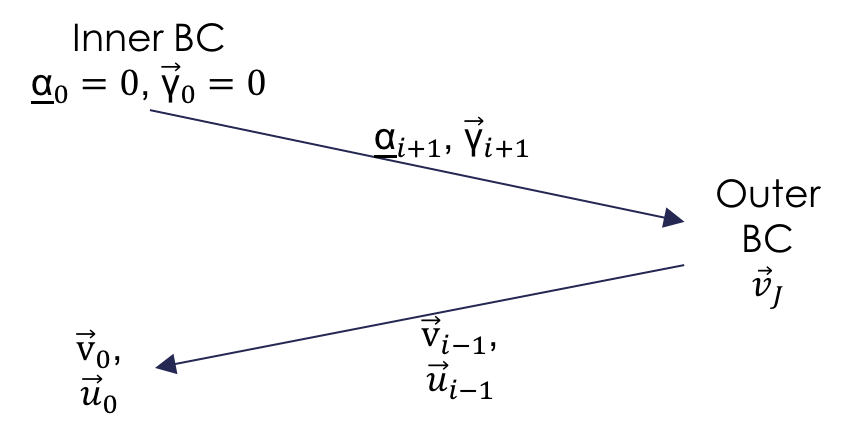
\includegraphics[width = 0.5 \textwidth]{figures/Overview.png}
\caption{A diagrammatic overview of the Henyey method, showing what is being evaluated at each stage of the code.  The arrows represent the two recurrence relations, with the inwards arrow progressively calculating the solution as it works back towards the centre of the grid.}
\end{center}
\end{figure}


This code was built from scratch, and tested extensively in various situations, particularly assessing the differences between analytically equivalent expressions of the recurrence relations and the differences between different applications of the boundary conditions.  The numerical components were also extensively tested, including ensuring the accuracy of matrix and vector manipulation, particularly matrix inversion in the case of small determinants; a structure to deal with the manipulation of complex numbers was included and tested; and a method of interpolation of input data was built, such that the maximum cell size could be precisely controlled and varied across the grid.  These were used to solve a variety of different equations, ranging from simple algebraic equations up to the complex differential equations which are used to solve the stellar oscillation equations.







\section{Implementing the equations}  \label{Implement}

This section discusses the more specific implementation of the stellar oscillation equations, including the problems associated with that, and how they were addressed and overcome.

\subsection{Choosing the form of the equations}  \label{Implement:Form}

Once a general Henyey code has been successfully built and tested, the first stage in applying it to a specific problem is to change the equations which it is solving.  However, this is not a simple task, as the form of the equations and the precise form of the variables which are being solved for affects the accuracy of the code.  The primary thing to avoid is for any variable, term, or matrix component to be divided by anything which goes to $0$.  It is important to be mindful of the fact that the term is split over the course of the solution, and that checking that the equation itself has no poles is insufficient.

As such, in making the equations and variables dimensionless, I avoided dividing anything by $r$, $g_{0}$, $F_{r_{0}}$, or any other variable which goes to $0$ at any point.  This resulted in the normalisations of variables as:

\begin{align}
\tilde{\xi}_{r} &\equiv \frac{\xi_{r}}{R} \\
\tilde{F}_{r} &\equiv \frac{F_{r}}{F_{r_{BC}}} \\
\tilde{p} &\equiv \frac{p}{p_{0}} \\
\tilde{T} &\equiv \frac{T}{T_{0}}
\end{align}
\\
where $F_{r_{BC}} = F_{r_{0}} |_{r=R}$.  This, combined with the careful treatment of the oscillation equations, was found to converge well to the solution when used with dummy test cases where the answers are fully known analytically.



\subsection{Discretisation}   \label{Implement:Disc}

The code does not directly take the equations as an input, but rather takes the form of the matrices $A$ to $H$, the vectors $M$ and $N$ (as well as the corresponding matrices and vectors in the outer boundary condition).  Therefore the equations must be expressed in a discretised form, but efforts must be made to minimise the loss of accuracy as a result of this.

The primary way of achieving this is to be very careful about where variables are defined, and where the equations are being evaluated.  To determine where each equation is being evaluated, one must consider which derivatives are present in the equation, and one must only use variables from cells $k$ and $k+1$.  For equation \ref{eq:ACD} this is the centre of cell $k+1$, and is therefore fairly simple: the cell-centre variables are simply given by their $k+1$ value, the cell-face variables are given by a simple average of the $k$ and $k+1$ values.  For equation \ref{eq:EFH}, however, things are not so simple, as this equation must be evaluated at the face of cell $k$, and adjacent cells need not be the same size.  Although most adjacent cells will be of a similar size, on some occasions, such as towards the very centre or outer edge of the star, the cell size may vary rapidly in size.  In this case, the cell-face variables are simply given by their $k$ value, but the cell-centre variables must be evaluated using a weighted average, essentially linearly interpolating between the two known values to estimate the value at the face of cell $k$.  It must be noted, however, that this scheme of averaging is only effective if the variables can be approximated well by a linear variation over the range of the two cells, which necessitates a sufficiently fine grid.

The derivatives as a whole must also be treated carefully.  In an attempt to prevent introducing extra sources of numerical inaccuracy, derivatives of multiple variables are, where possible, expressed as a single derivative, rather than expanding the term using the chain rule.  Whilst this may have some drawbacks in cases of different size cells where the derivative is non-linear (although this would again be minimised by increasing the resolution), it is more stable against potential poles in any individual variable involved in the derivative.



\subsection{Input data}   \label{Implement:Input}

As the equations work by perturbing an equilibrium model of the star, the code requires that this equilibrium state be provided as an input.  As mentioned in section \ref{Intro:StellarStruc}, this stellar model is created using MESA.  Once created, data about the properties of the star can be extracted and formatted to be used as an input for the Henyey code, and with this the variables are already split into cell-centre and cell-face types, and the data is output on a discrete grid.  This defines the underlying grid for the implementation of the Henyey code, but is insufficient for our purposes.

In order to use this data in a satisfactory manner, the grid must be made sufficiently fine across the whole star, with particularly fine resolution in areas which give a highly spatially oscillatory response (that is expected to be the radiative regions, where solutions are expected to be oscillatory, whereas the are expected to be evanescent in convective zones).  This requires that new points be added to the grid, requiring both interpolating the input data, and controlling the maximum cell size throughout the star.

These two processes are obviously intimately related, as neither can effectively occur without the other.  The resolution is controlled by setting a maximum cell size as a function of position in the star, and splitting any cells which exceed that size.  The difficulty comes about when trying to split the cells whilst still keeping track of how the old arrays containing the input data correspond to the new, higher resolution, arrays which must be filled with accurately interpolated data.  Controlling the accuracy of the interpolation requires control of the process of generating the grid within MESA, by setting maximum changes in variables between adjacent cells to a suitable value such that the linear interpolation scheme is valid.  A particular problem with this is the fact that the parts of the star that MESA requires highest resolution for are not necessarily the parts which the Henyey code requires highest resolution for, particularly for central radiative zones, which MESA regards as simple to model, but in which the very highest (spatial) frequency oscillations occur.  Another potential problem is the fact that cell-centre variables, in order to be strictly interpolated rather than extrapolated, are not simply a weighted average of their $k-1$ and $k$ values, but, for adding cells to the outer half of a cell, require interpolating between $k$ and $k+1$.  This asymmetry in the interpolation of cell-centre variables compared to cell-face variables could potentially lead to artificially large derivatives evaluated in the new, finer grid.  However, we must once again rely upon the choice of the skeleton grid from MESA being appropriate (or once again, to rely on our controls to make it so), so that the change in variables between adjacent cells is kept within a reasonable limit such that this effect is controlled.



\subsection{Other considerations}   \label{Implement:Other}

I will outline some other problems in the implementation of the Henyey code to solve the oscillation equations here, particularly focussing on how they were overcome, or worked around.


In choosing the form of the recurrence relations used in the Henyey code, multiple different expressions for analytically equivalent versions were possible.  A major consideration was to ensure that inverting singular matrices (such as using $\underline{\alpha}_{0}^{-1}$) was avoided, which limited the possible sensible range of expressions.  Even so, these different expressions were tested to discover which versions were most effective in solving the test equations, and how to express them using the fewest matrix manipulations.  For the outgoing recurrence relation, there was only one essential expression, and all the others were found to be exactly analytically equivalent.  For the returning recurrence relation, however, two genuinely distinct options are available.  Both cases were tested and their accuracy evaluated, and case I was selected to be used.  Further details can be found in appendix \ref{ap:Henyey}.


A major obstacle to achieving the required resolution was the limitation due to the size of the available RAM.  This is a result of the fact that the process to iterate from step $k+1$ to $k$ on the return journey requires information which was used to step from $k$ to $k+1$ on the outgoing journey.  As such, each step is not stand-alone, and a large amount of memory was being used in defining each matrix at each location in the star for the entirety of the calculation.  In order to improve this situation, I introduced some new arrays which would be used specifically to exactly what would be needed for the return journey, and only that information.  Using this, each matrix array need only contain the information for the step from $k$ to $k+1$ at the time that that outward step is being evaluated, as the required information for the step from $k+1$ to $k$ on the return journey would be evaluated at that point and saved, then the matrices would be re-evaluated for the next outward step.  This introduces a few arrays of dimension $2 \times 2 \times J$, but also cuts down many arrays from the previously required $2 \times 2 \times J$ to $2 \times 2 \times 2$.  This solution does still hit another limit, however, as there are still some matrices which grow linearly with the resolution, so the RAM limitation is still in place, but at a suitable resolution.  Also, as the resolution is controlled as a function of position in the star, the limited number of cells can be distributed such that the highest resolution is where the need is greatest, although this is not an automatic process, but must be managed manually.







\section{Output}

In order to ensure that the code and equations are all correct, work from a previous paper (Terquem \textit{et al}, 1998, figure 1) has been reproduced and the output has been compared.  The previous work used a shooting method, and treated the non-adiabatic case slightly differently, but good agreement has been found between the paper's result and my own, which can be seen in figure \ref{fig:non-ad}.  Some particular differences to note are the following: the precise form of spatial oscillations in the core varies depending on the exact parameters used in the solution (which will be explored in the following paragraphs), and the behaviour at the very surface (that is, the last $\sim 0.1 \%$ of the star's radius) is significantly different, although this is due to the thin outermost radiative layer of the star, and is not thought to be a problem with the Henyey method's application in this case.



\begin{figure}[htbp]
\begin{center}
\begin{subfigure}{0.5\textwidth}
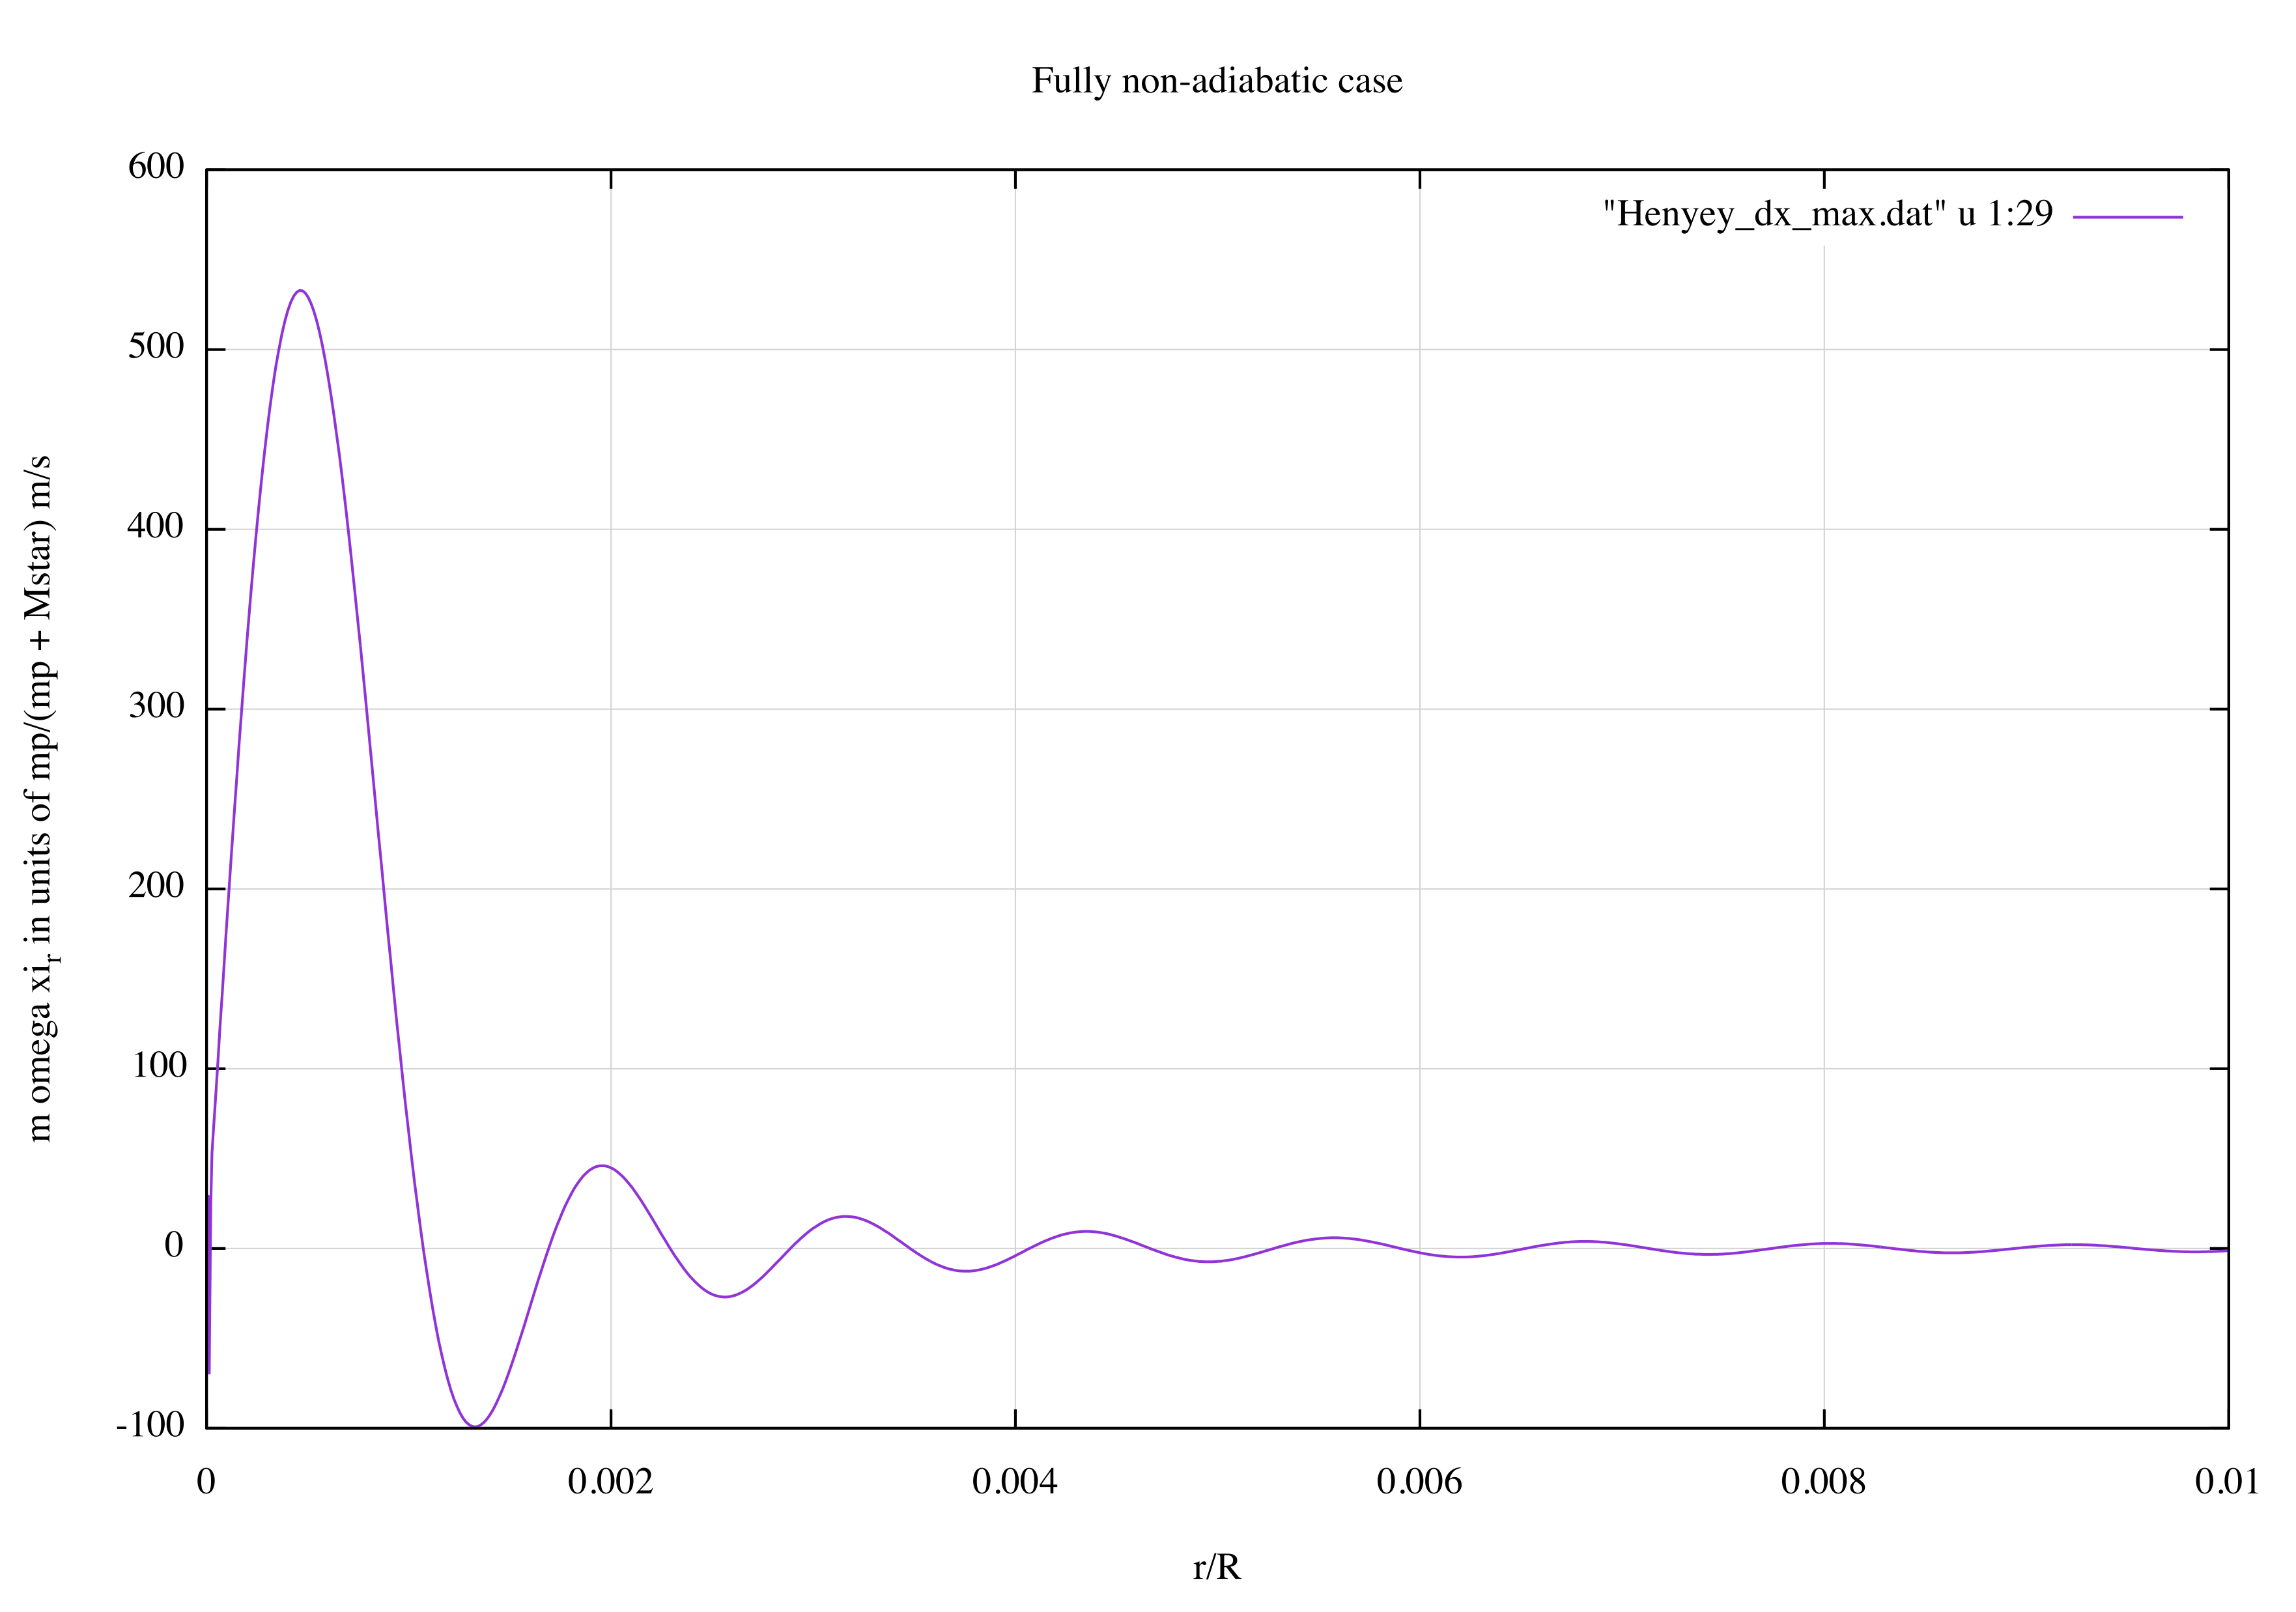
\includegraphics[width = \textwidth]{figures/xi_r_section1_non-ad.png}
\end{subfigure}
~
\begin{subfigure}{0.5\textwidth}
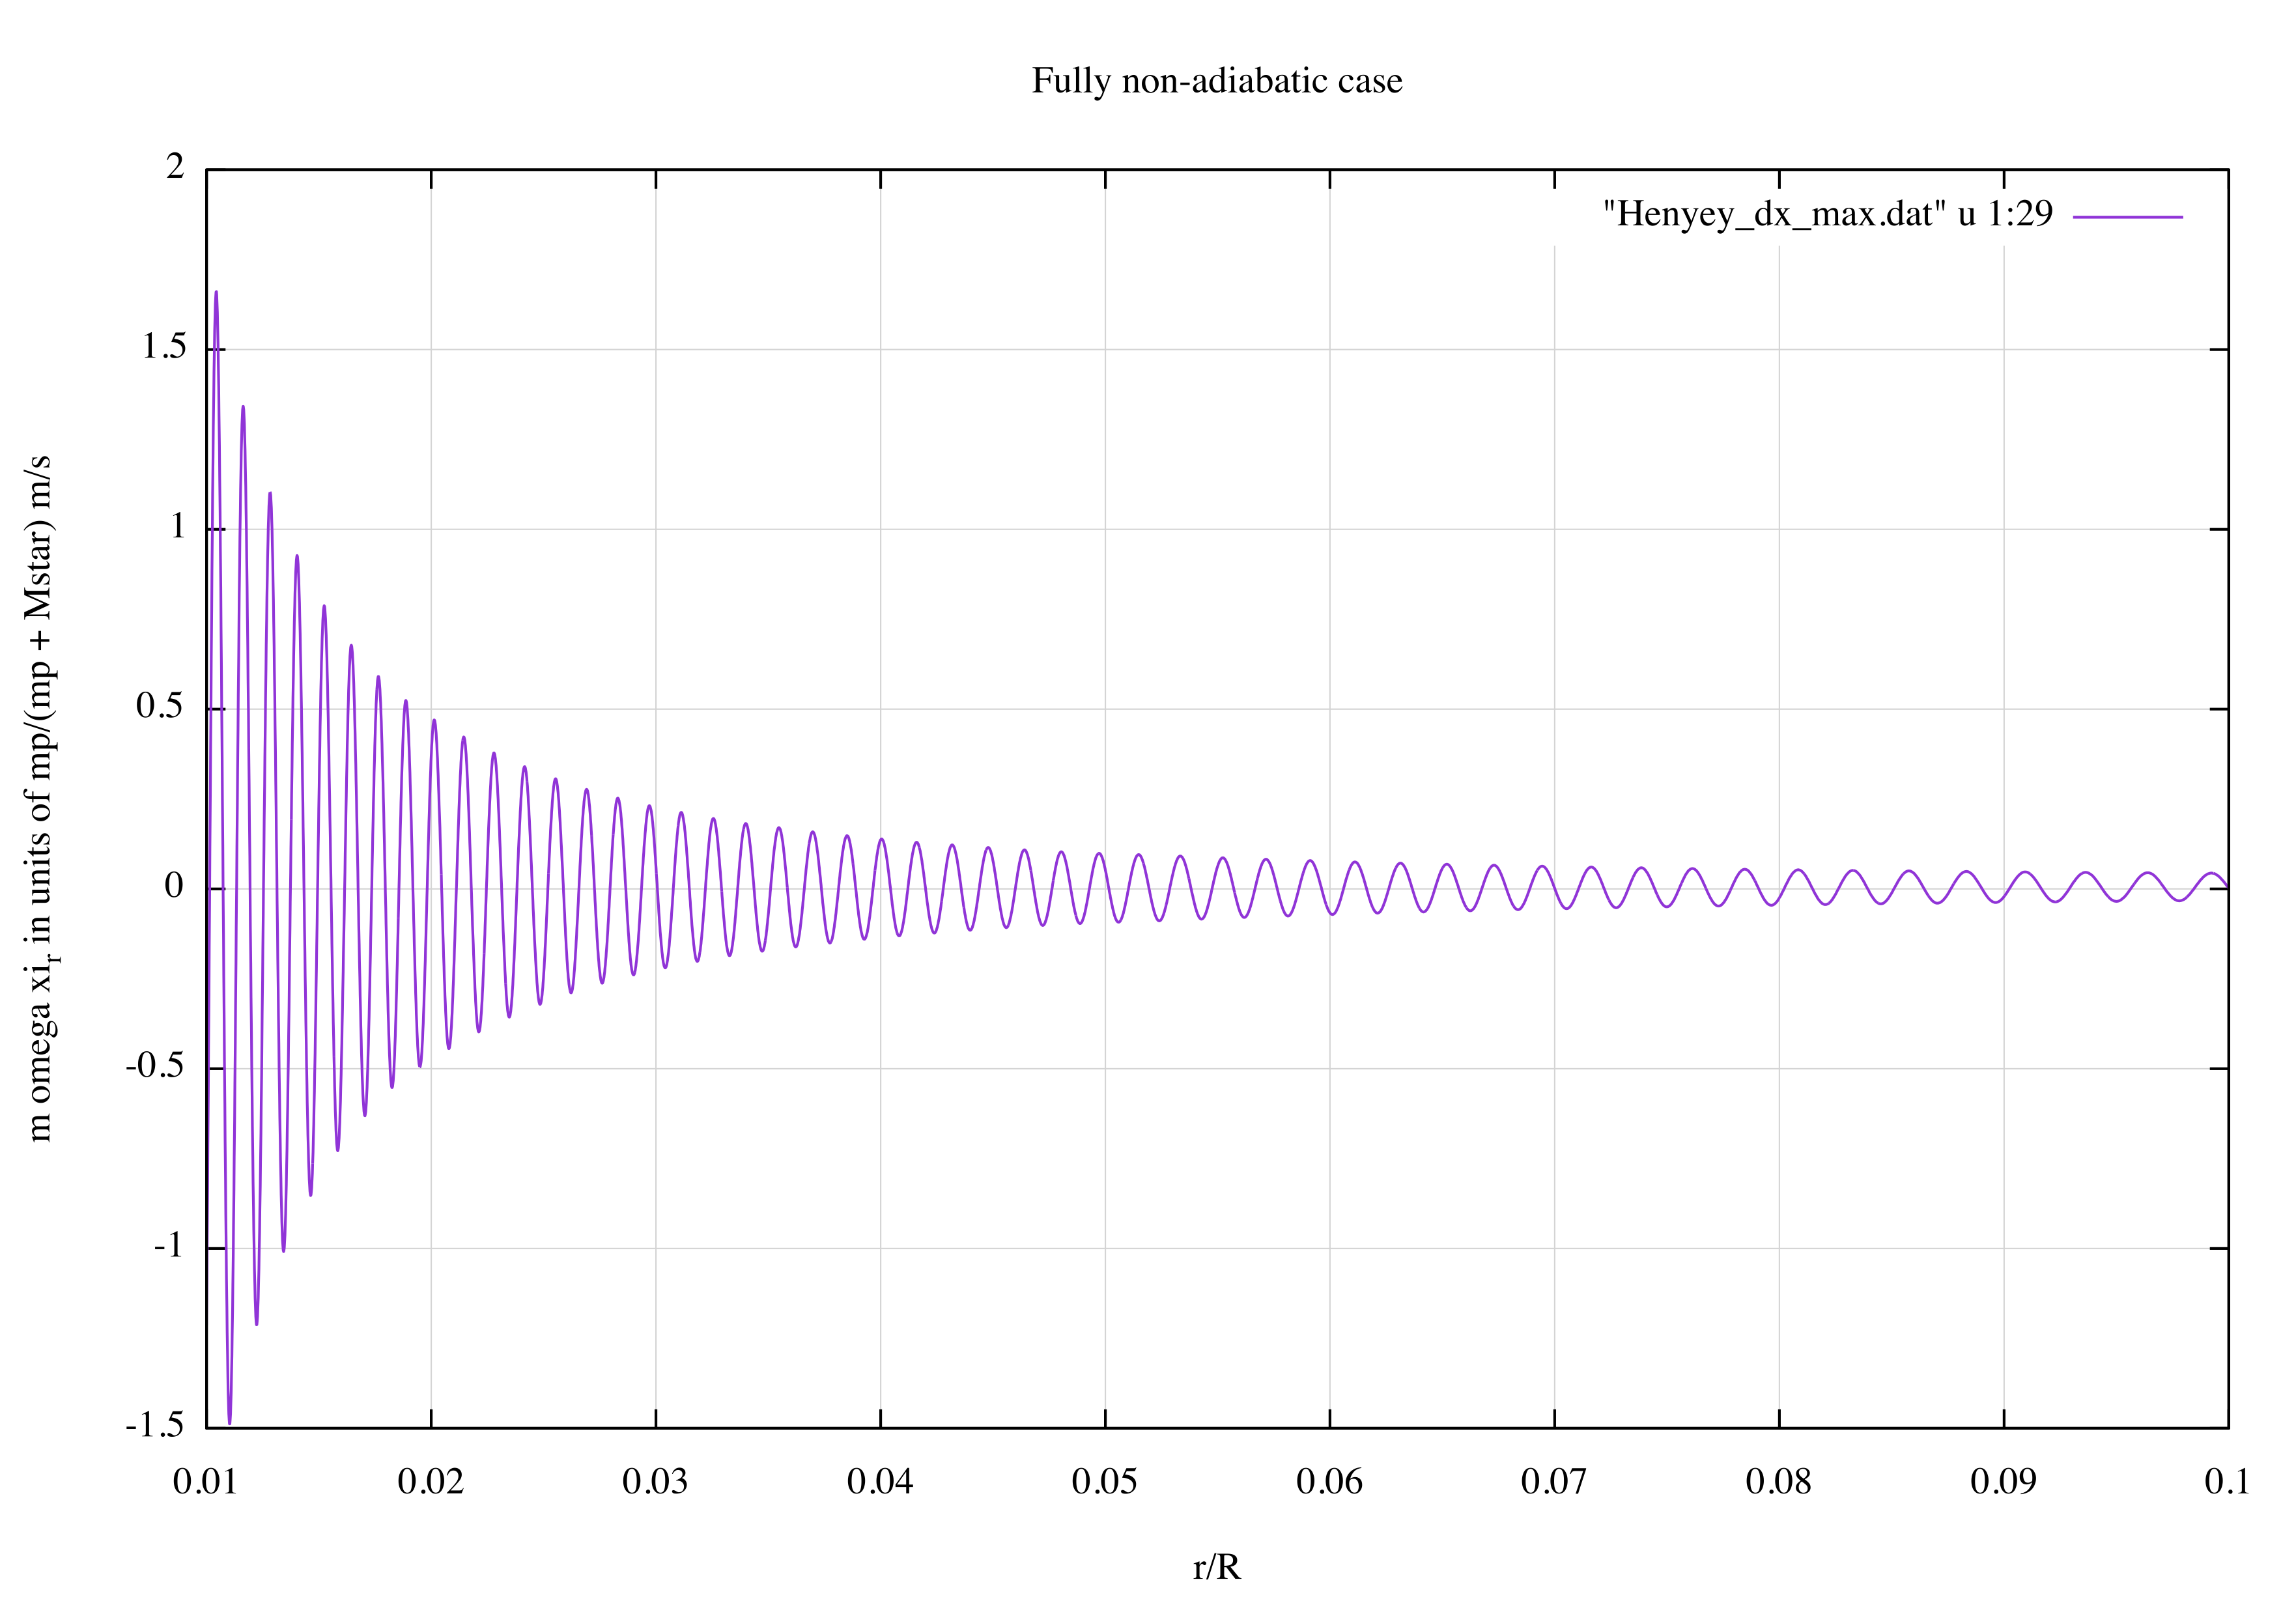
\includegraphics[width = \textwidth]{figures/xi_r_section2_non-ad.png}
\end{subfigure}

\begin{subfigure}{0.5\textwidth}
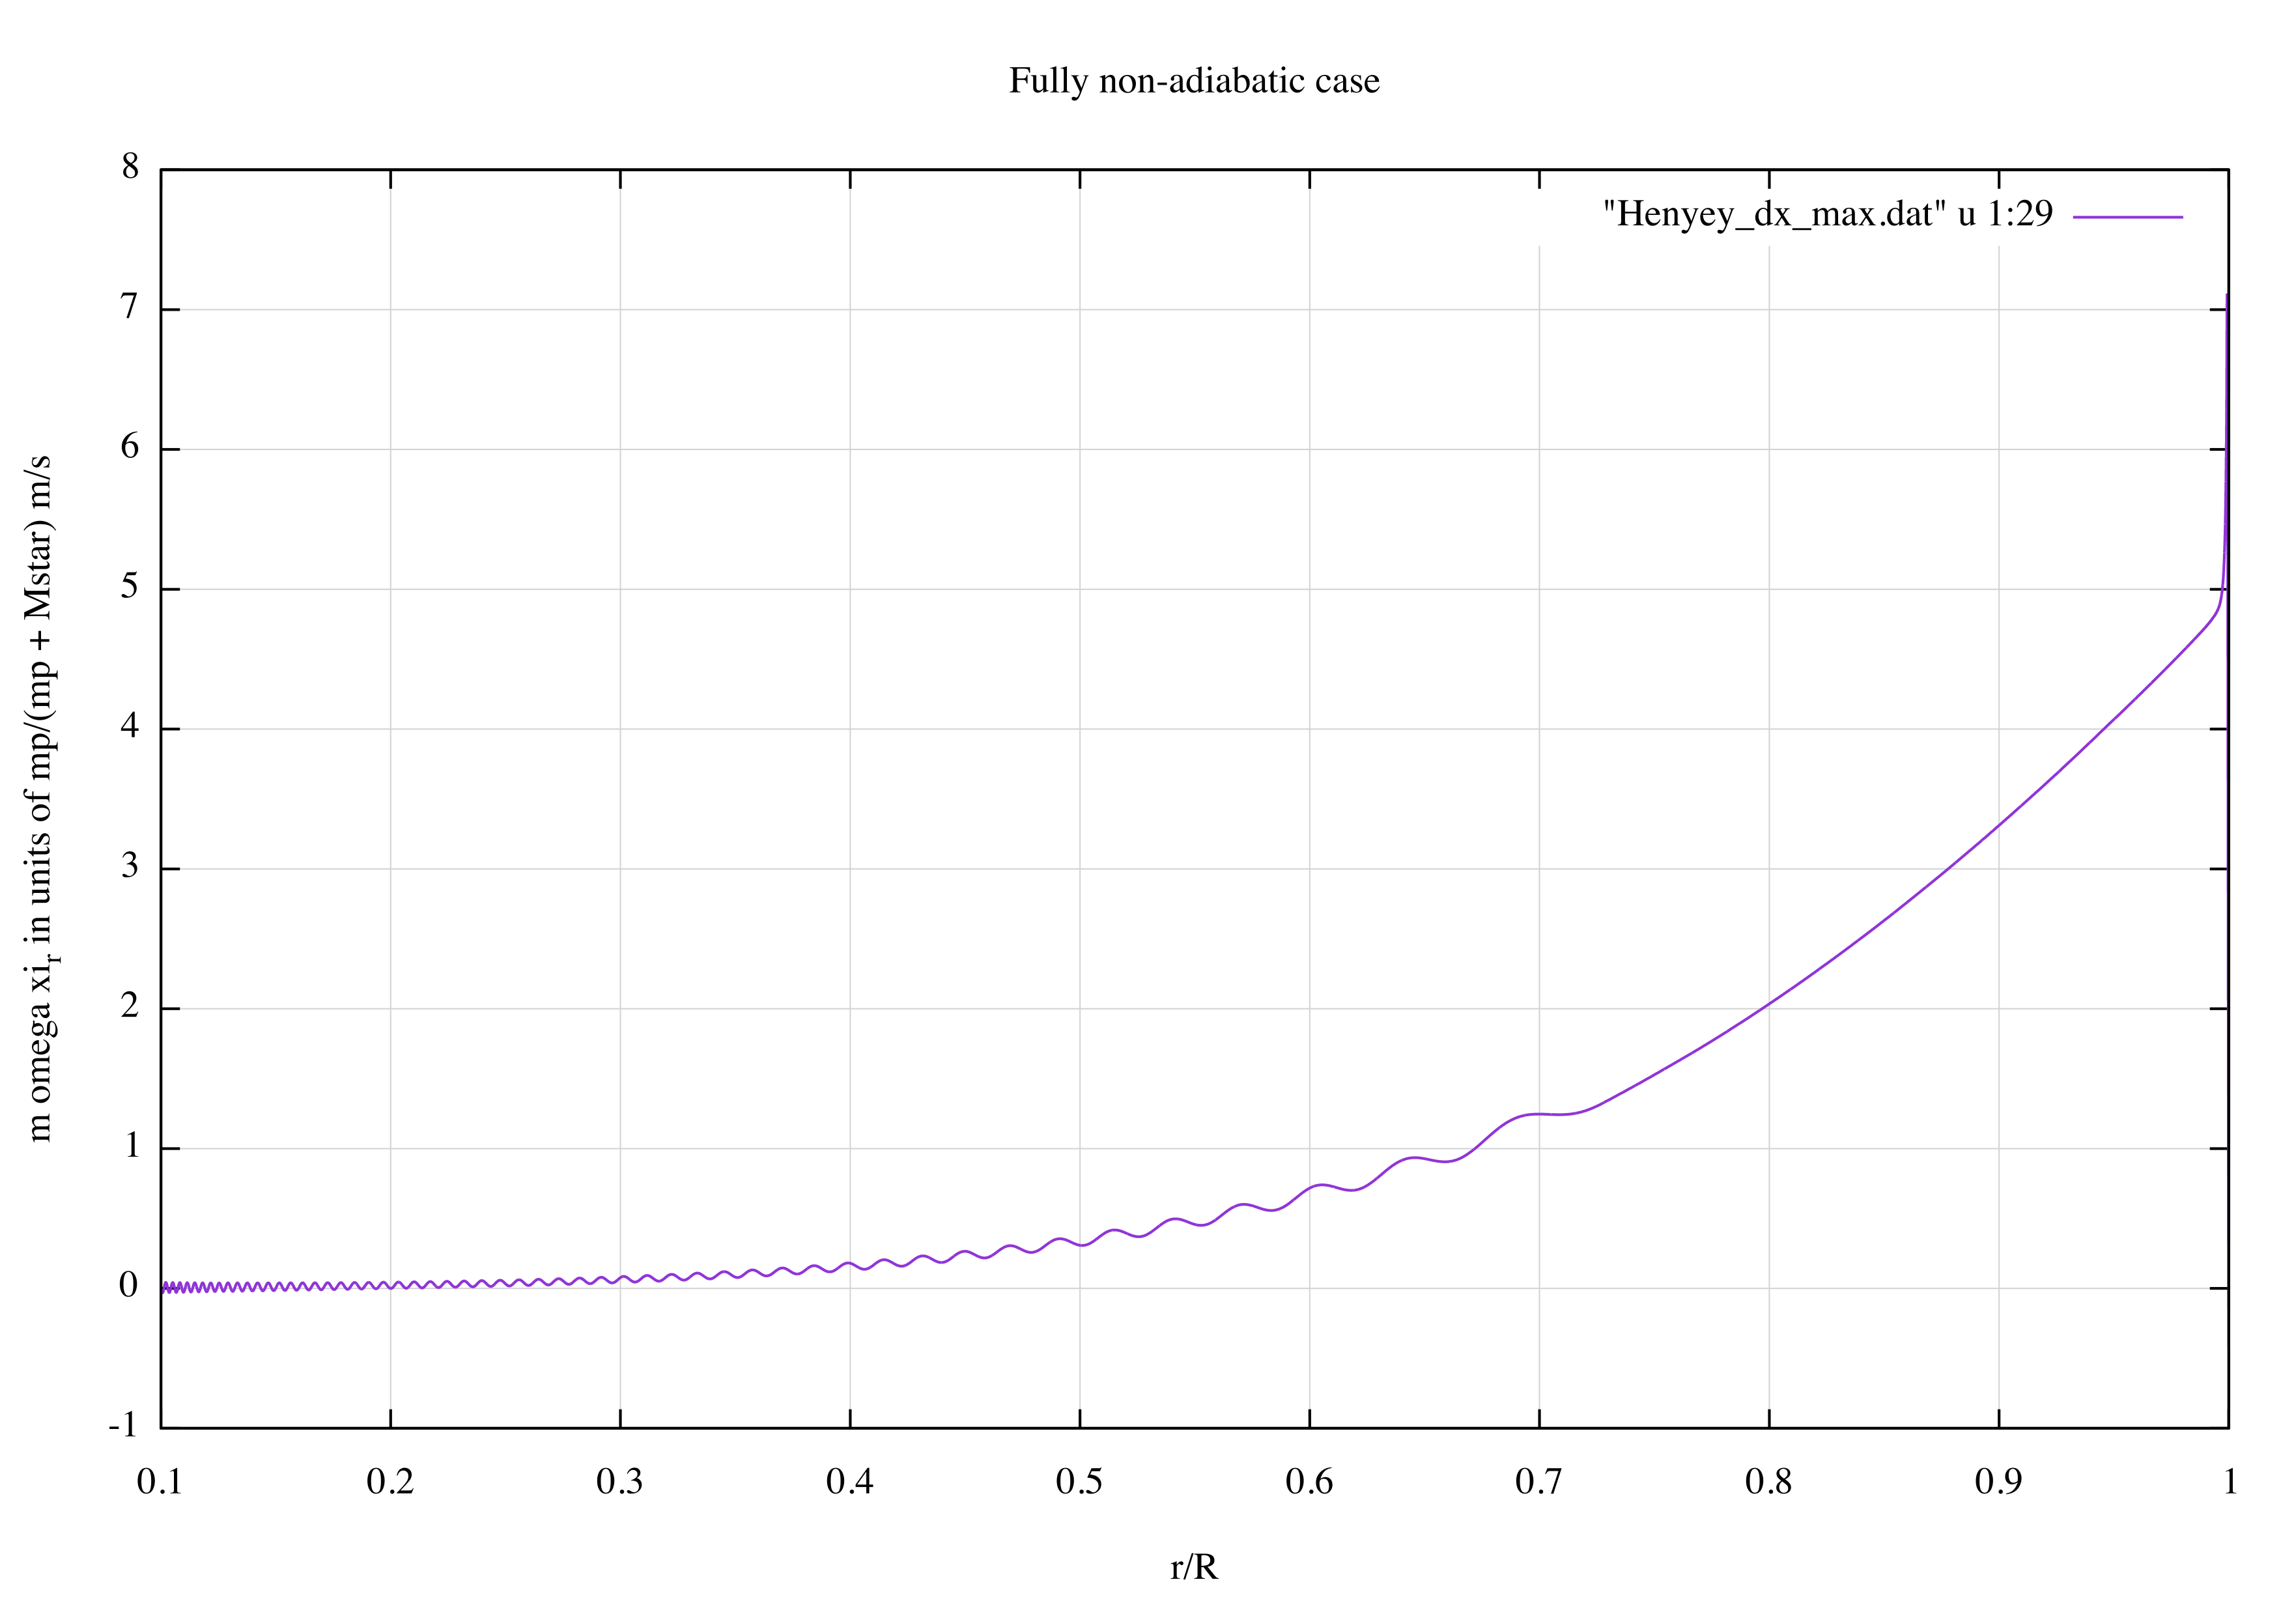
\includegraphics[width = \textwidth]{figures/xi_r_section3_non-ad.png}
\end{subfigure}
~
\begin{subfigure}{0.5\textwidth}
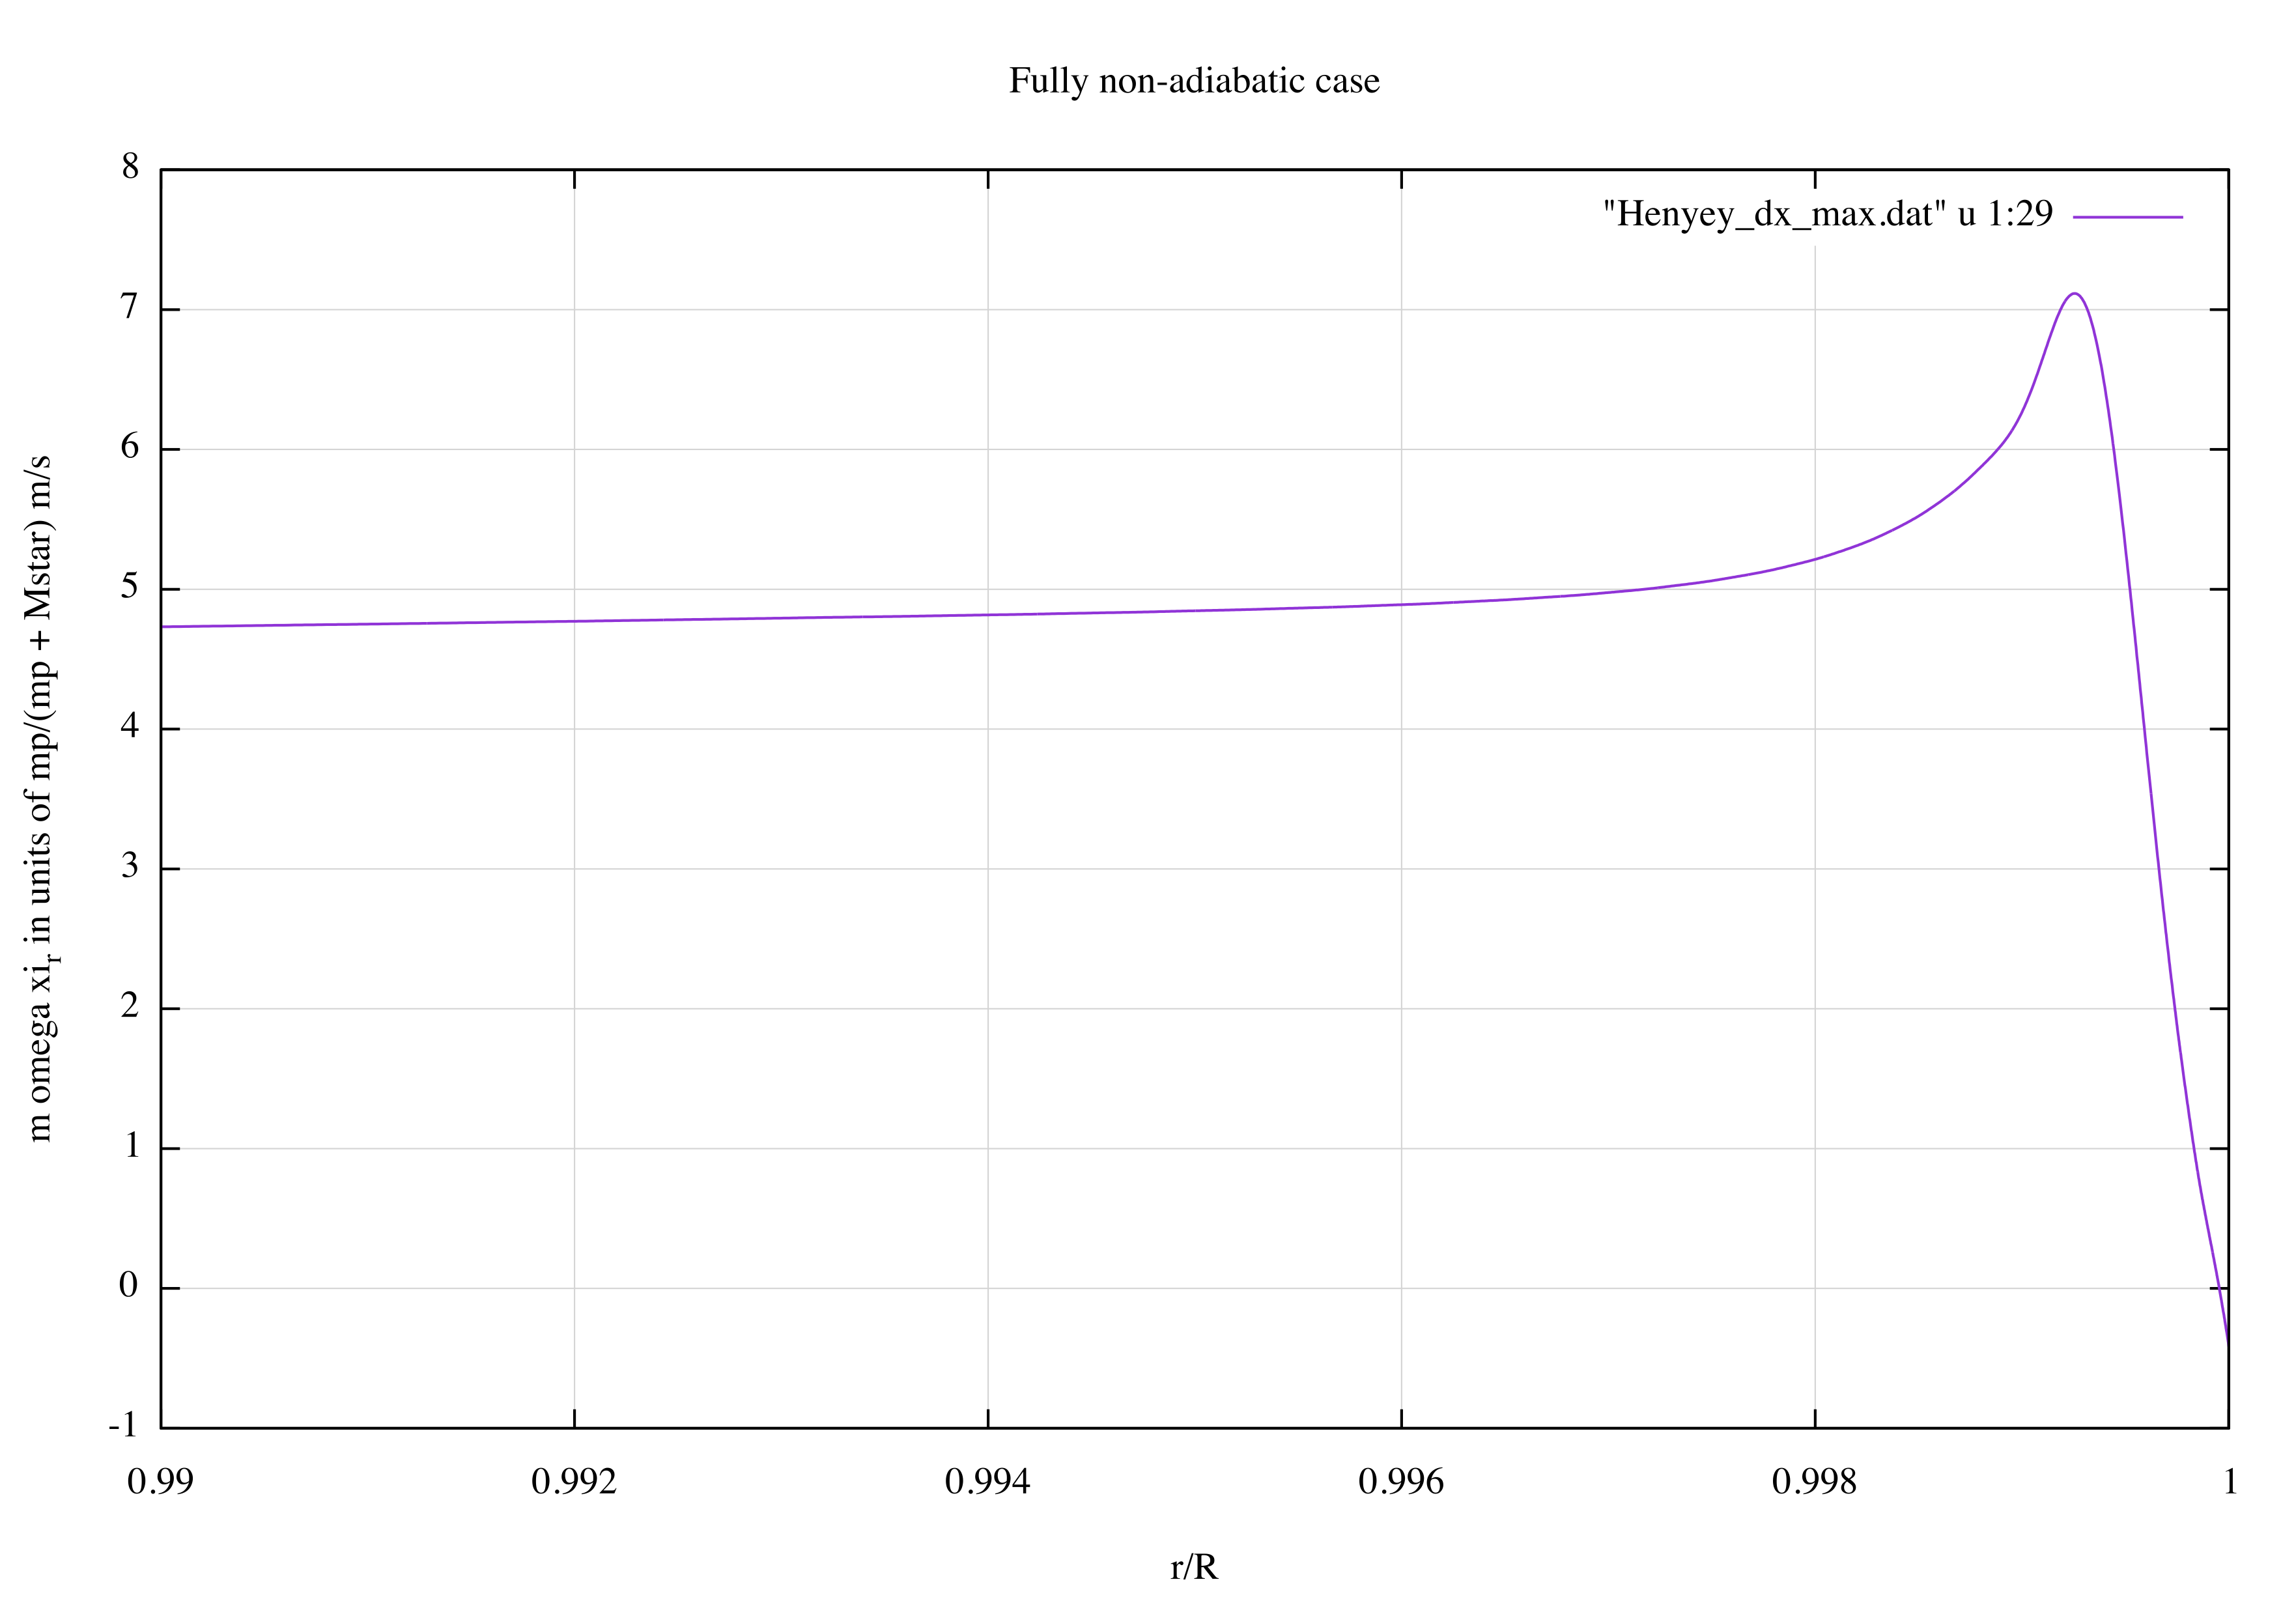
\includegraphics[width = \textwidth]{figures/xi_r_surface_non-ad.png}
\end{subfigure}

\caption{The full solution for the non-adiabatic case, showing the peak radial velocity (that is, $m \omega \xi_{r}$) in units of $\frac{m_{p}}{m_{p} + M_{*}}$ m s$^{-1}$, against the proportional radial distance from the centre.  Four segments have been shown, as the first three reproduce the graphs in Terquem \textit{et al}, 1998, and the fourth highlights the behaviour in the thin radiative layer at the star's surface.  As a rough guide, the y-axis is approximately in mm s$^{-1}$}
\label{fig:non-ad}
\end{center}
\end{figure}



To investigate some of the limitations of this solution, some of the parameters used in the solution were varied slightly, to investigate what effect this had in the different regions of the star.

Firstly, a purely physical parameter was varied by up to $1 \%$, the semi-major axis of the planet's orbit.  This would be expected to have a slight effect on the amplitude of the response throughout the star, as a more distant planetary companion would lead to a lessened tidal effect, but it would also slightly shift the frequency of the orbit, and would therefore be expected to alter the spatial frequency of oscillations within the star.  This effect can be seen in figure \ref{fig:Dvar}, where it is particularly notable that the amplitude of the spatial oscillations at the very centre varies hugely, from, effectively, $-300$ to $+500$ mm s$^{-1}$.  The overall trend, however of oscillations which grow towards the centre of the core is clearly maintained, as is the decrease in spatial frequency further from the core.  The transition to evanescent waves in the convective envelope (from $\frac{r}{R} \approx 0.7$) is consistent across the cases, and is very similar in amplitude (particularly given that the magnitude of the tidal potential varies as $D^{-3}$).  Overall, it seems that the observable behaviour is not particularly sensitive to small variations in $D$ for this case, and that the patterns of behaviour in each region are unaffected, but that one should be wary of drawing precise quantitative conclusions about the oscillations in the core.





\begin{figure}[htbp]
\begin{center}
\begin{subfigure}{0.5\textwidth}
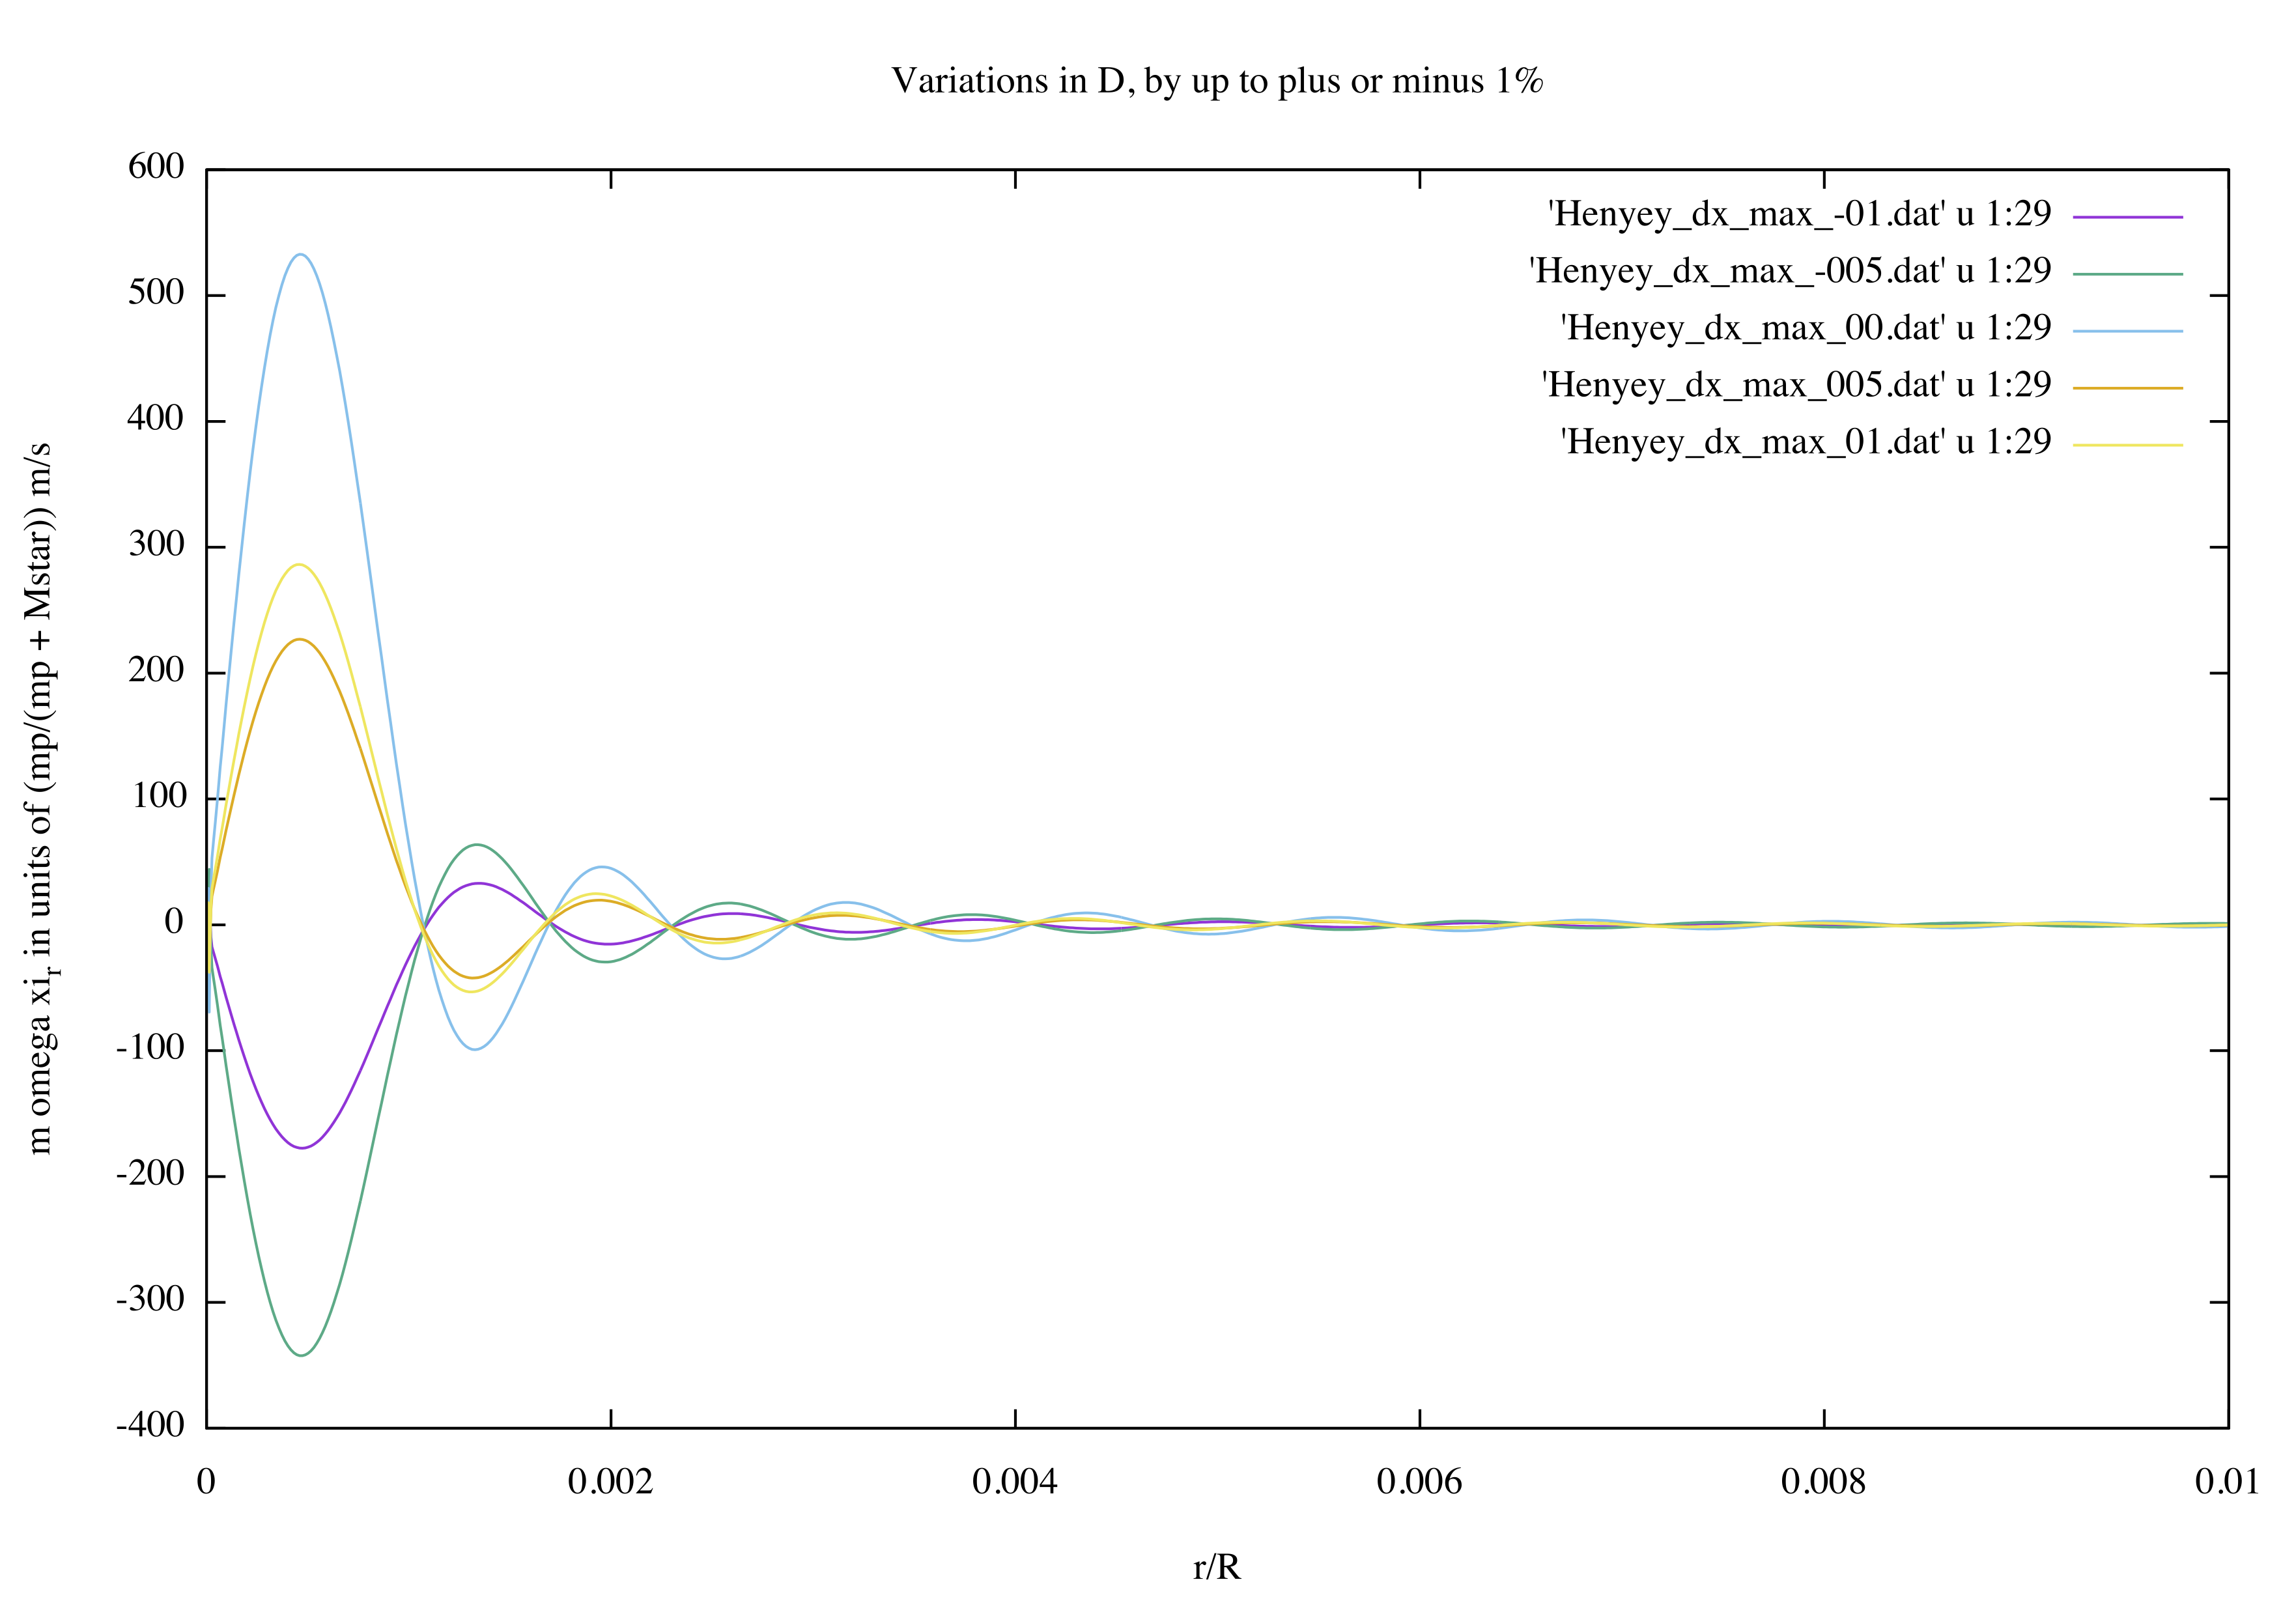
\includegraphics[width = \textwidth]{figures/xi_r_section1_Dvar.png}
\end{subfigure}
~
\begin{subfigure}{0.5\textwidth}
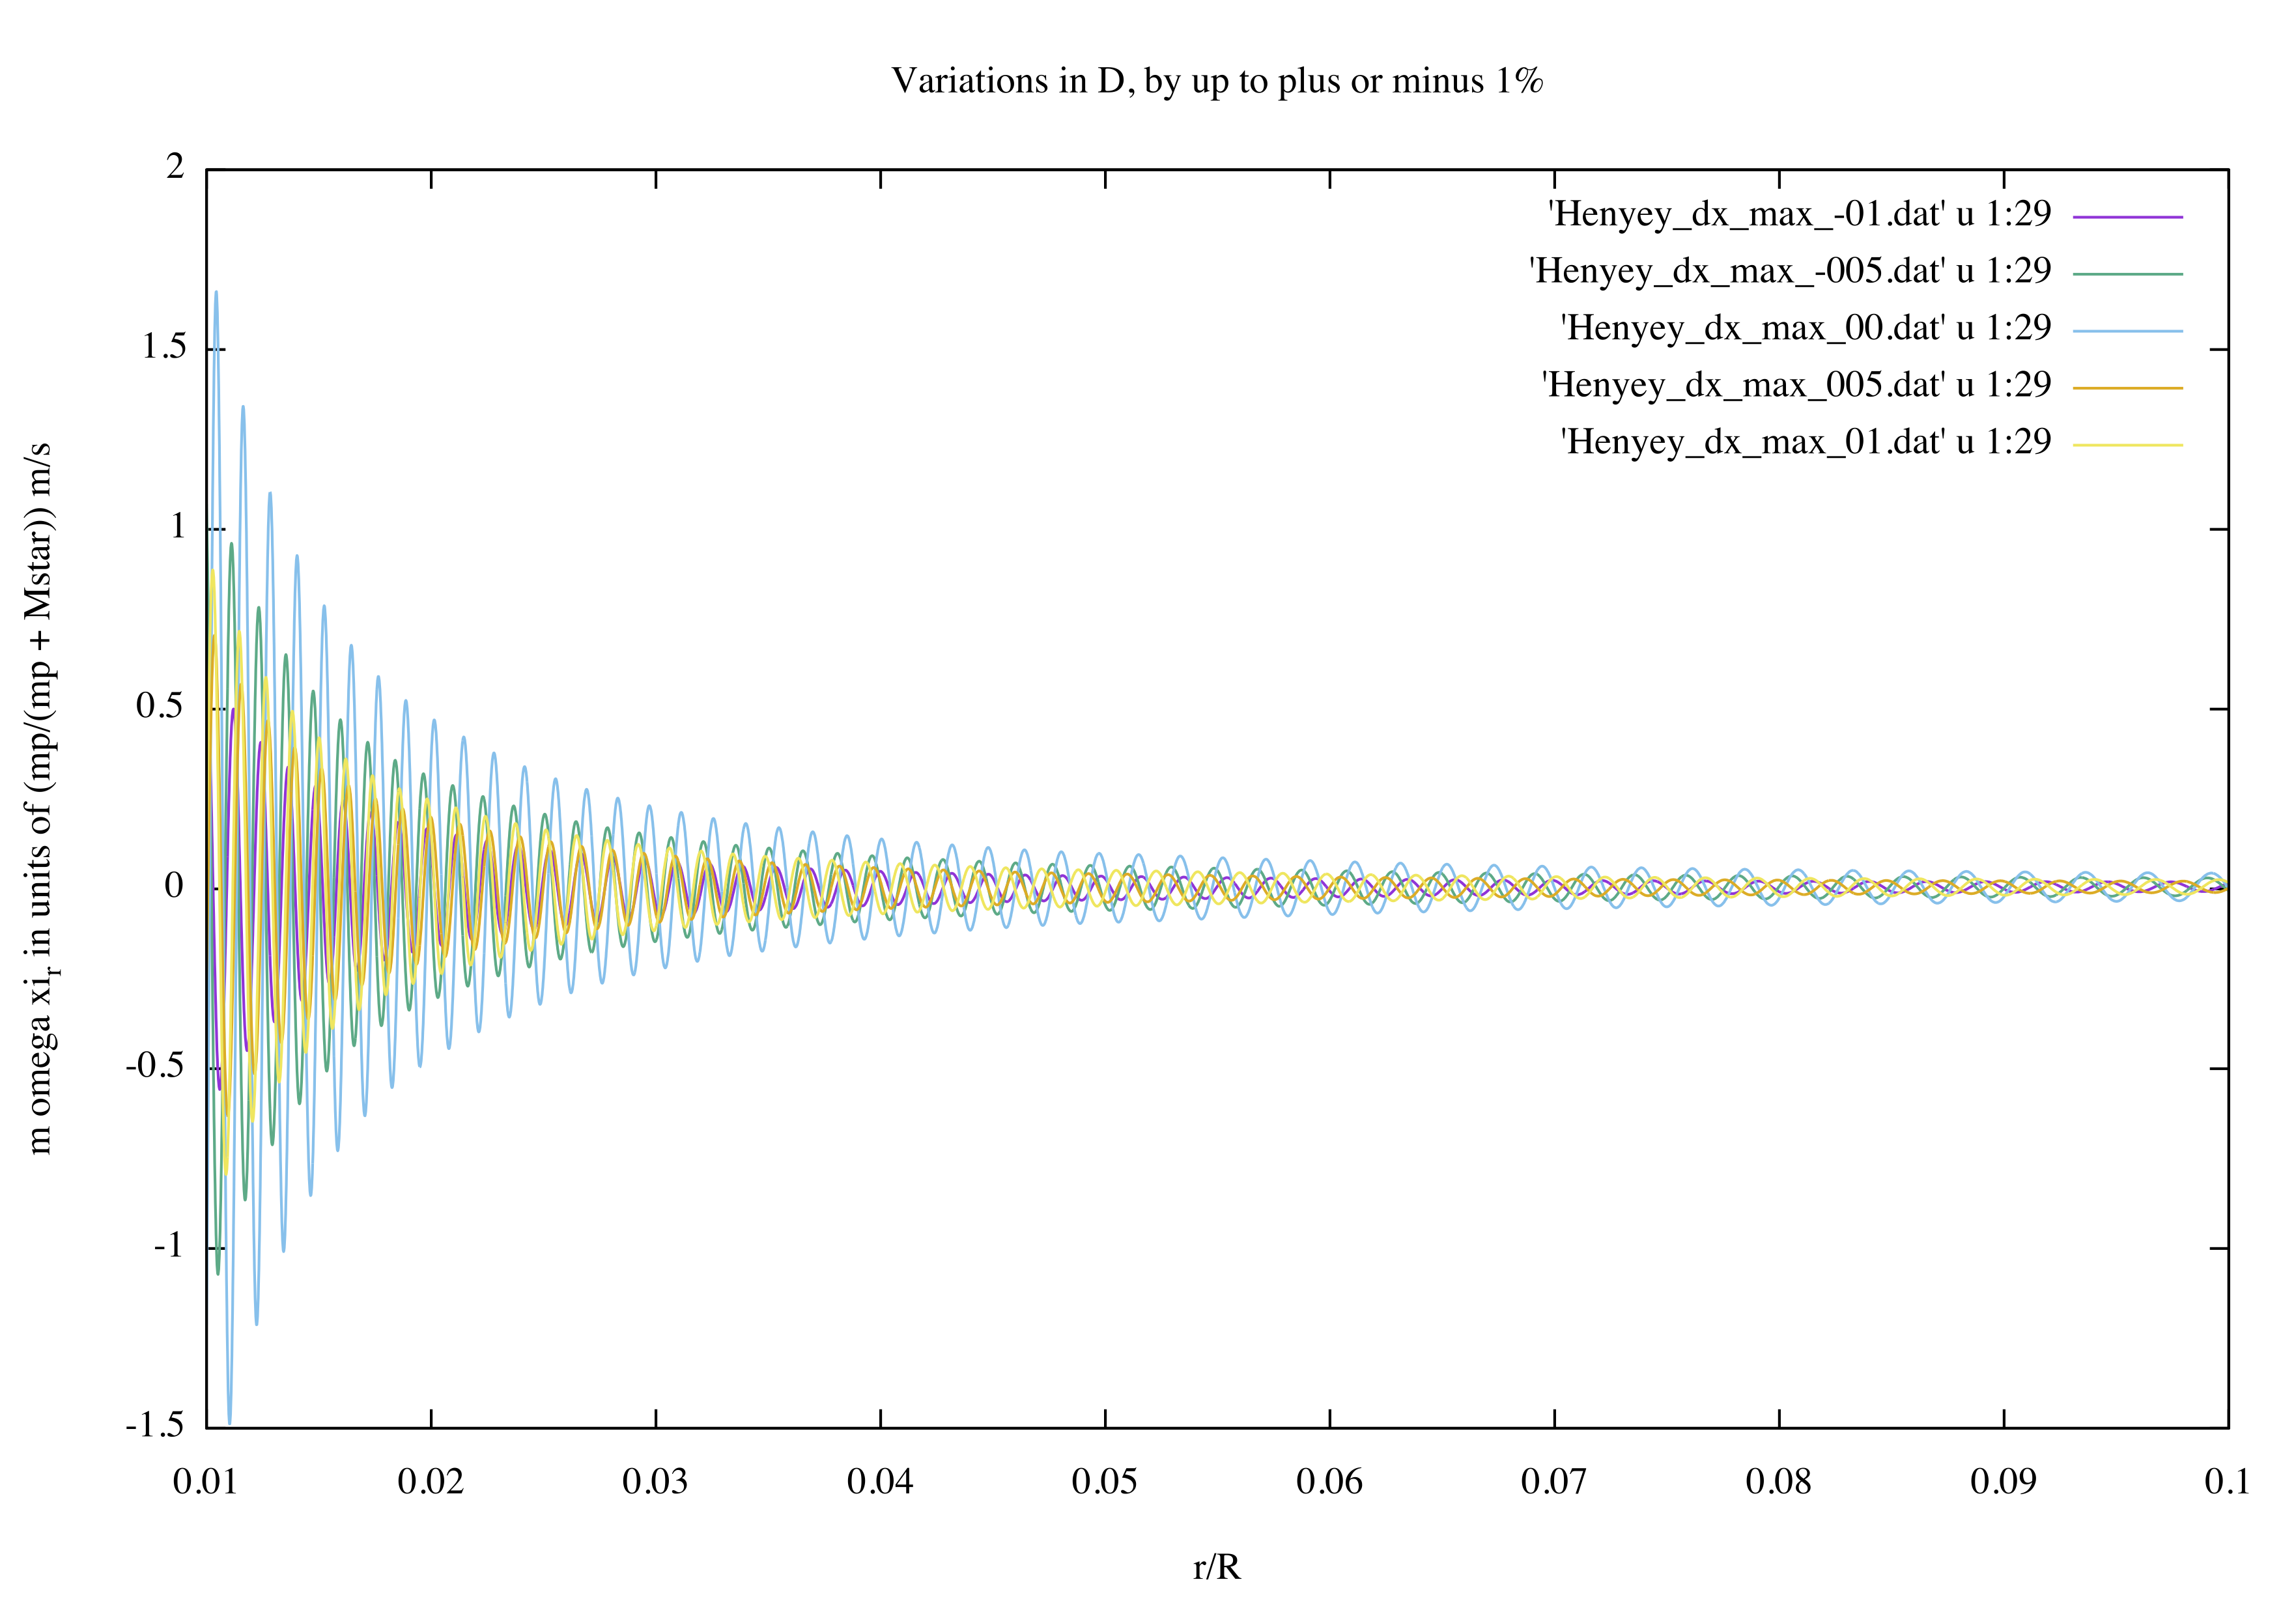
\includegraphics[width = \textwidth]{figures/xi_r_section2_Dvar.png}
\end{subfigure}

\begin{subfigure}{0.5\textwidth}
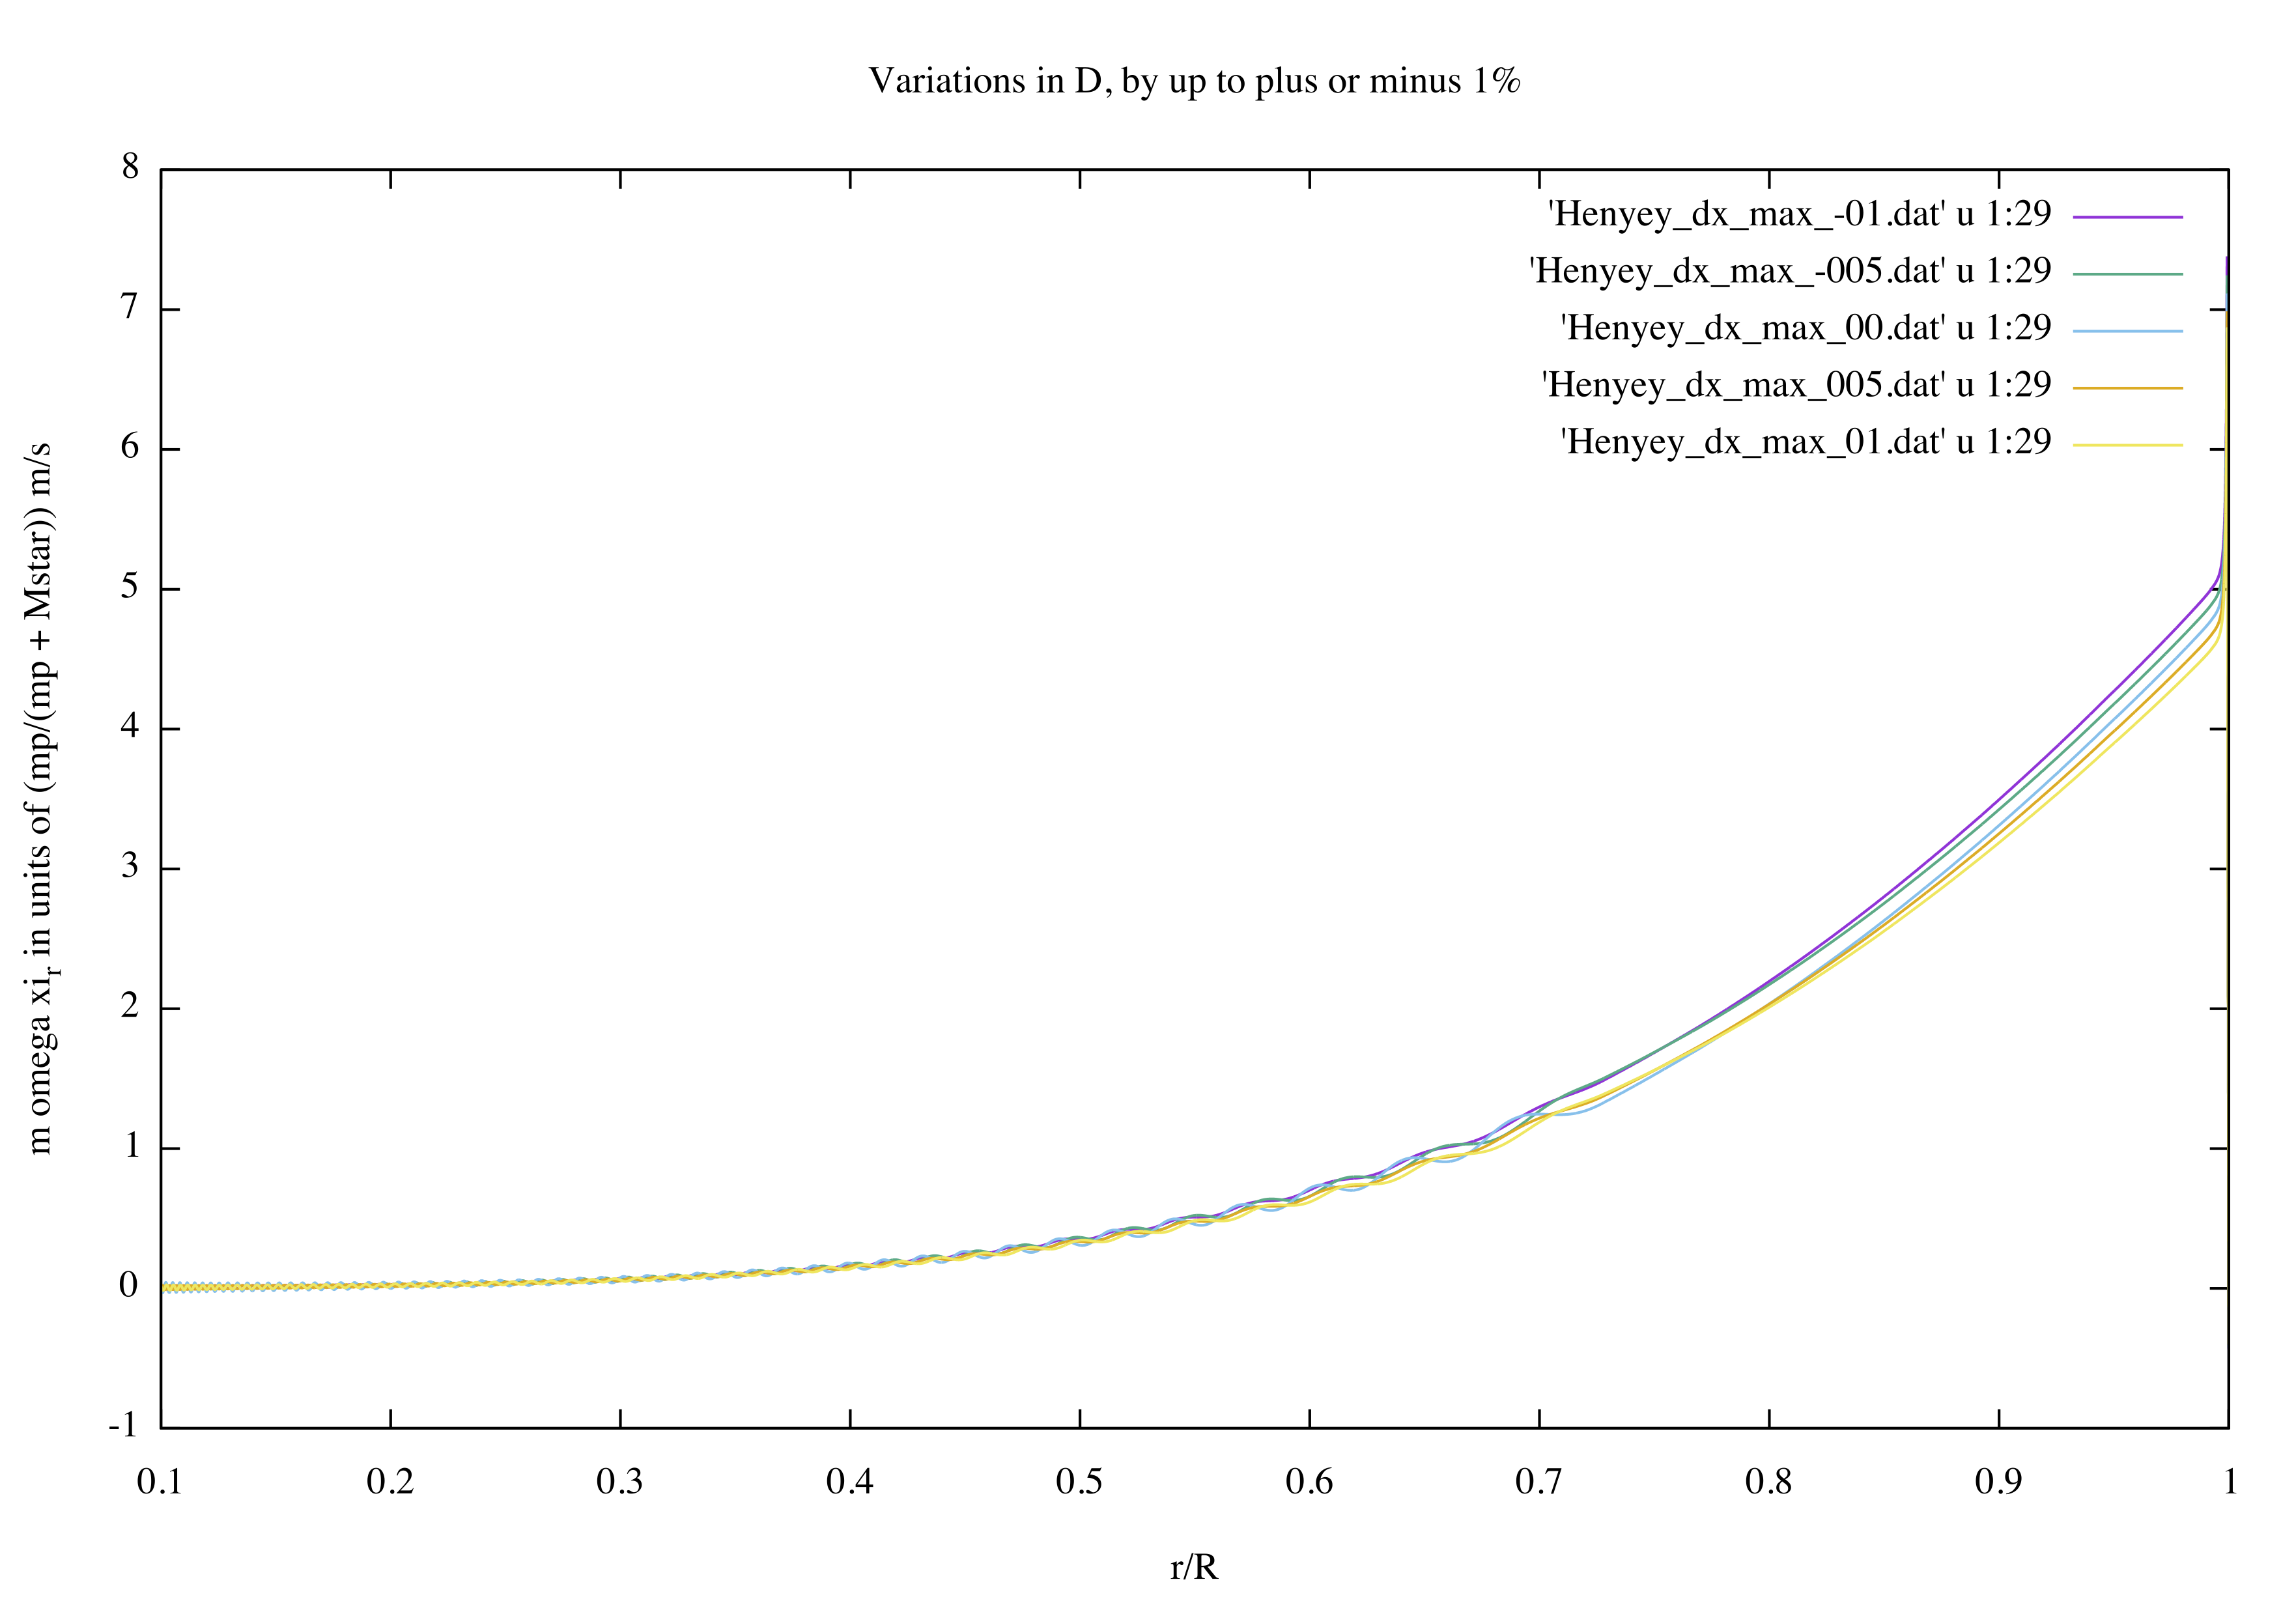
\includegraphics[width = \textwidth]{figures/xi_r_section3_Dvar.png}
\end{subfigure}
~
\begin{subfigure}{0.5\textwidth}
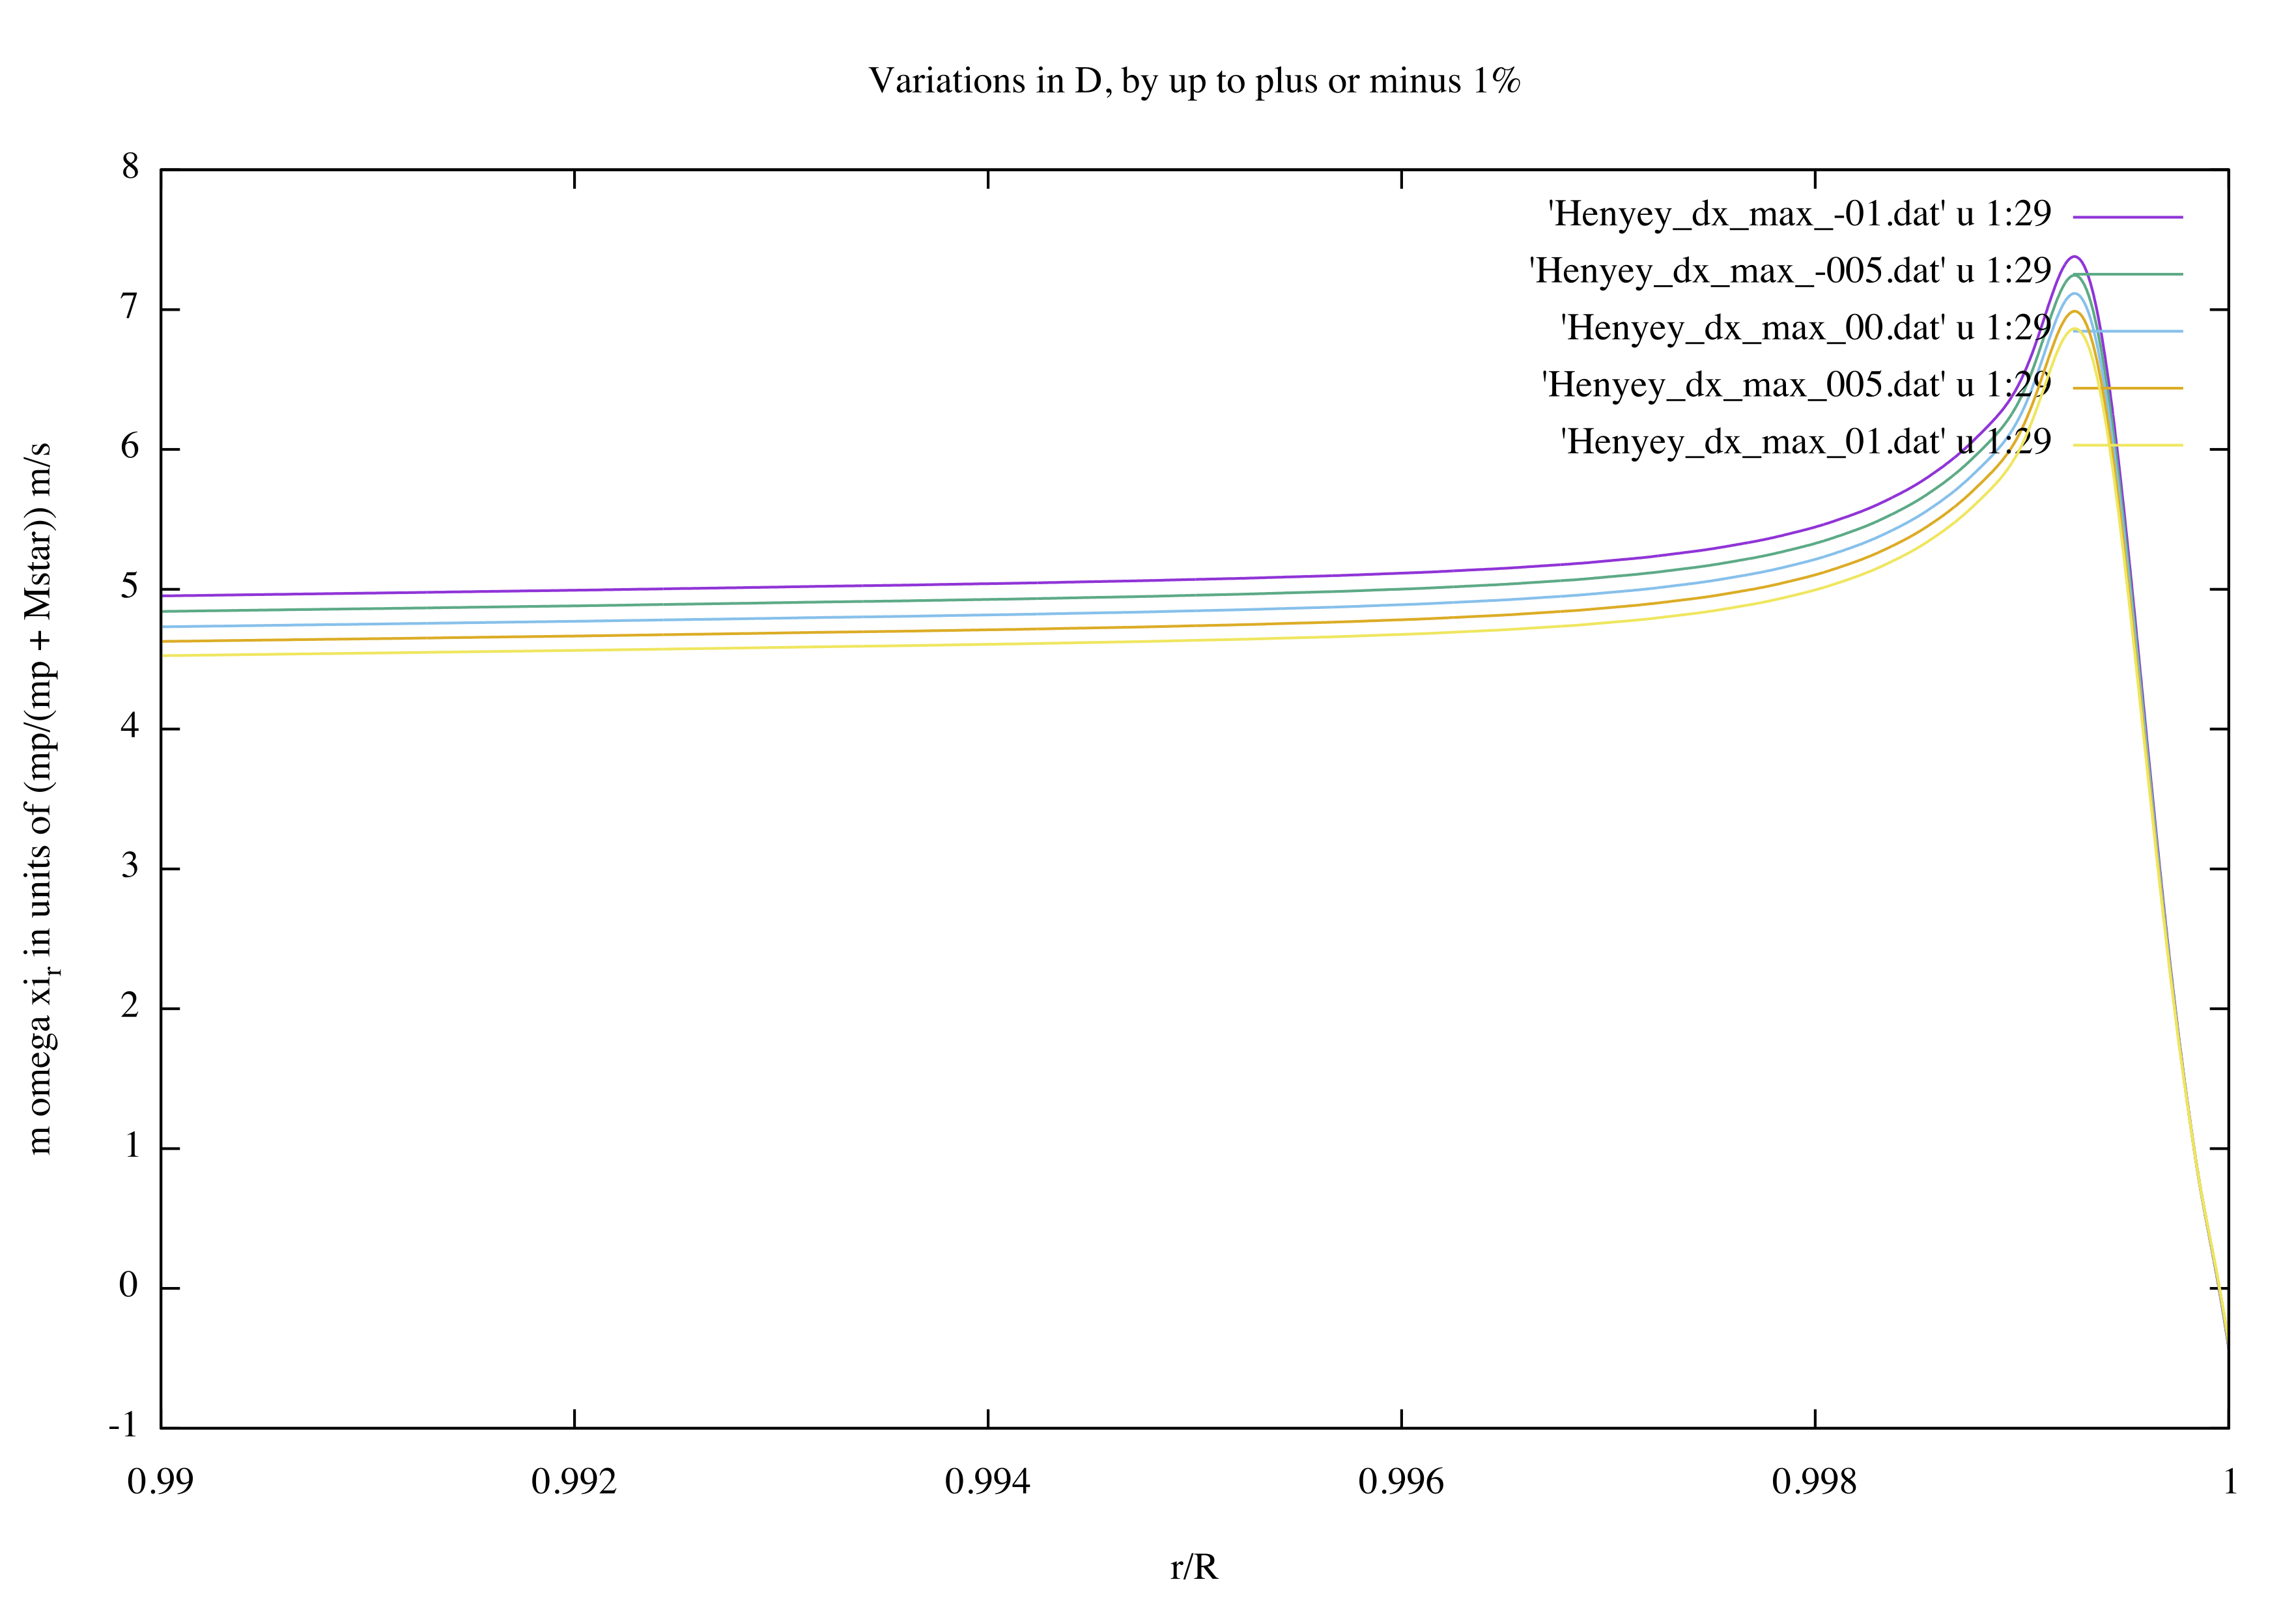
\includegraphics[width = \textwidth]{figures/xi_r_surface_Dvar.png}
\end{subfigure}

\caption{The full solution for the non-adiabatic case, showing the peak radial velocity (that is, $m \omega \xi_{r}$) in units of $\frac{m_{p}}{m_{p} + M_{*}}$ m s$^{-1}$, against the proportional radial distance from the centre.  In these figures, the semi-major axis of the planetary companion's orbit has been varied slightly, leading to a small spread in both the amplitudes and spatial frequencies of the oscillations.}
\label{fig:Dvar}
\end{center}
\end{figure}



The other parameter which was varied was the resolution.  In this case, a flat limit was introduced across the whole star, rather than varying it to match the needed resolution in order to try to keep things as simple as possible.




\begin{figure}[htbp]
\begin{center}
\begin{subfigure}{0.5\textwidth}
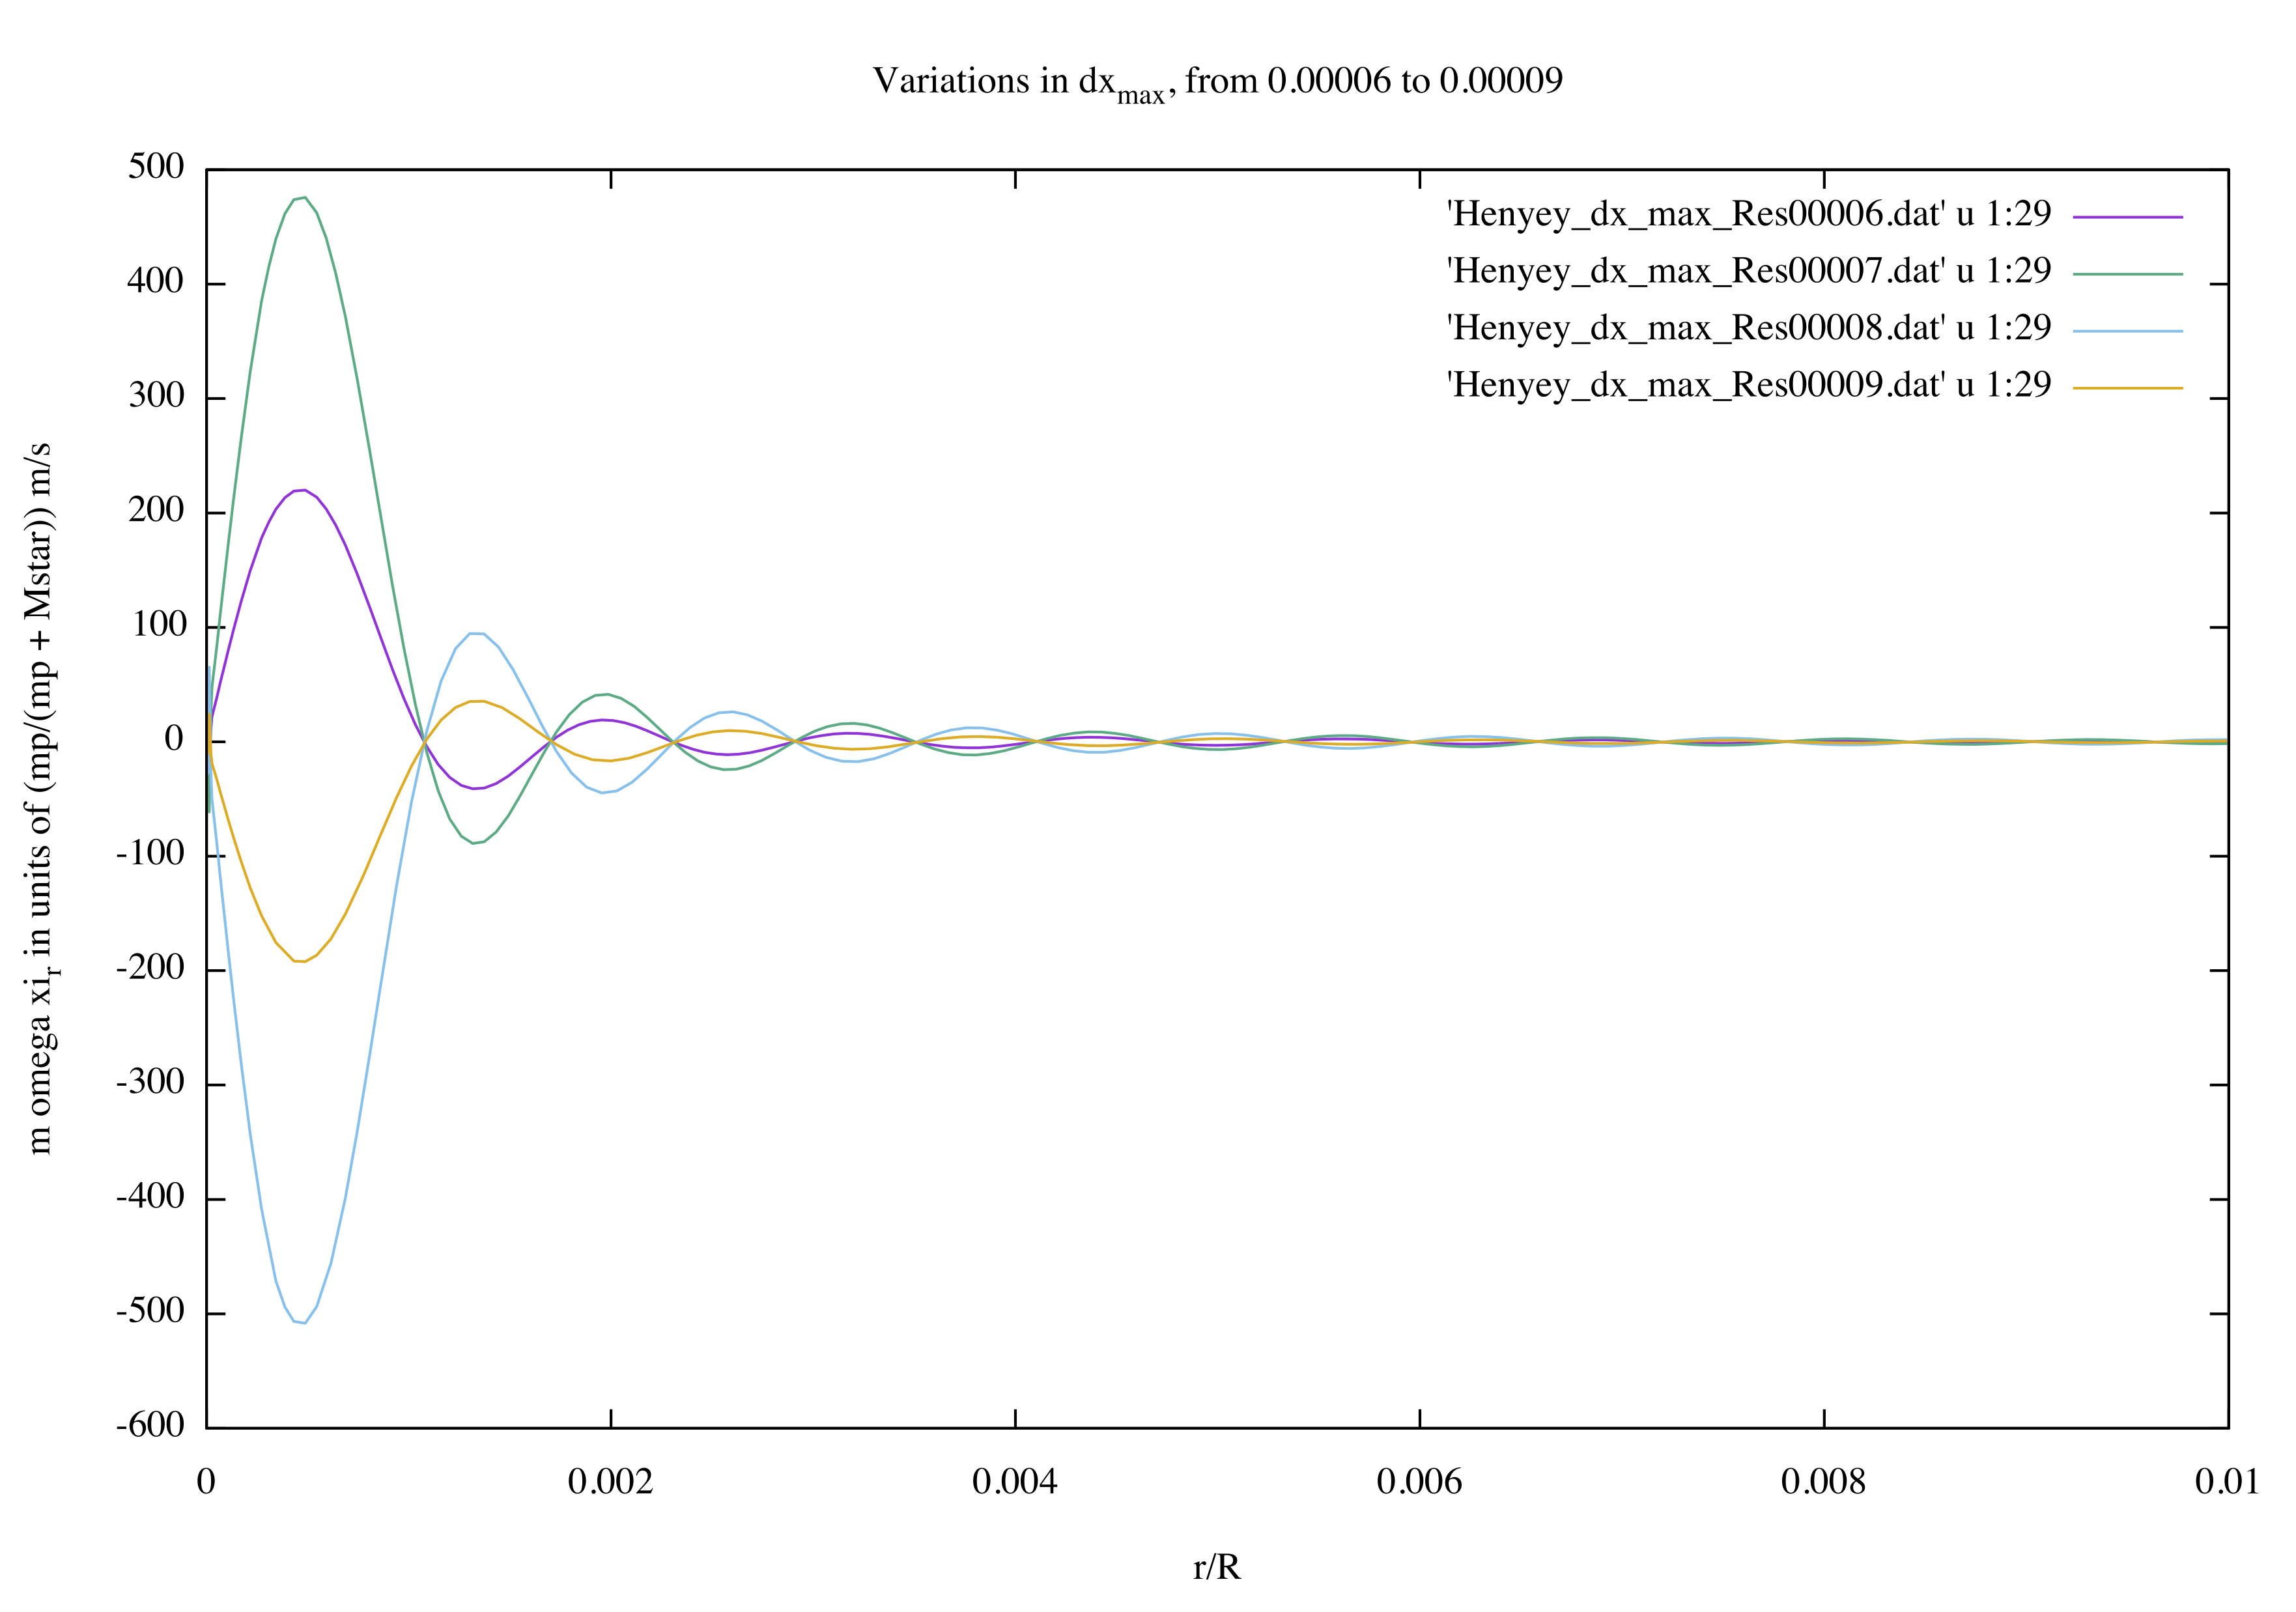
\includegraphics[width = \textwidth]{figures/xi_r_section1_Resvar.png}
\end{subfigure}
~
\begin{subfigure}{0.5\textwidth}
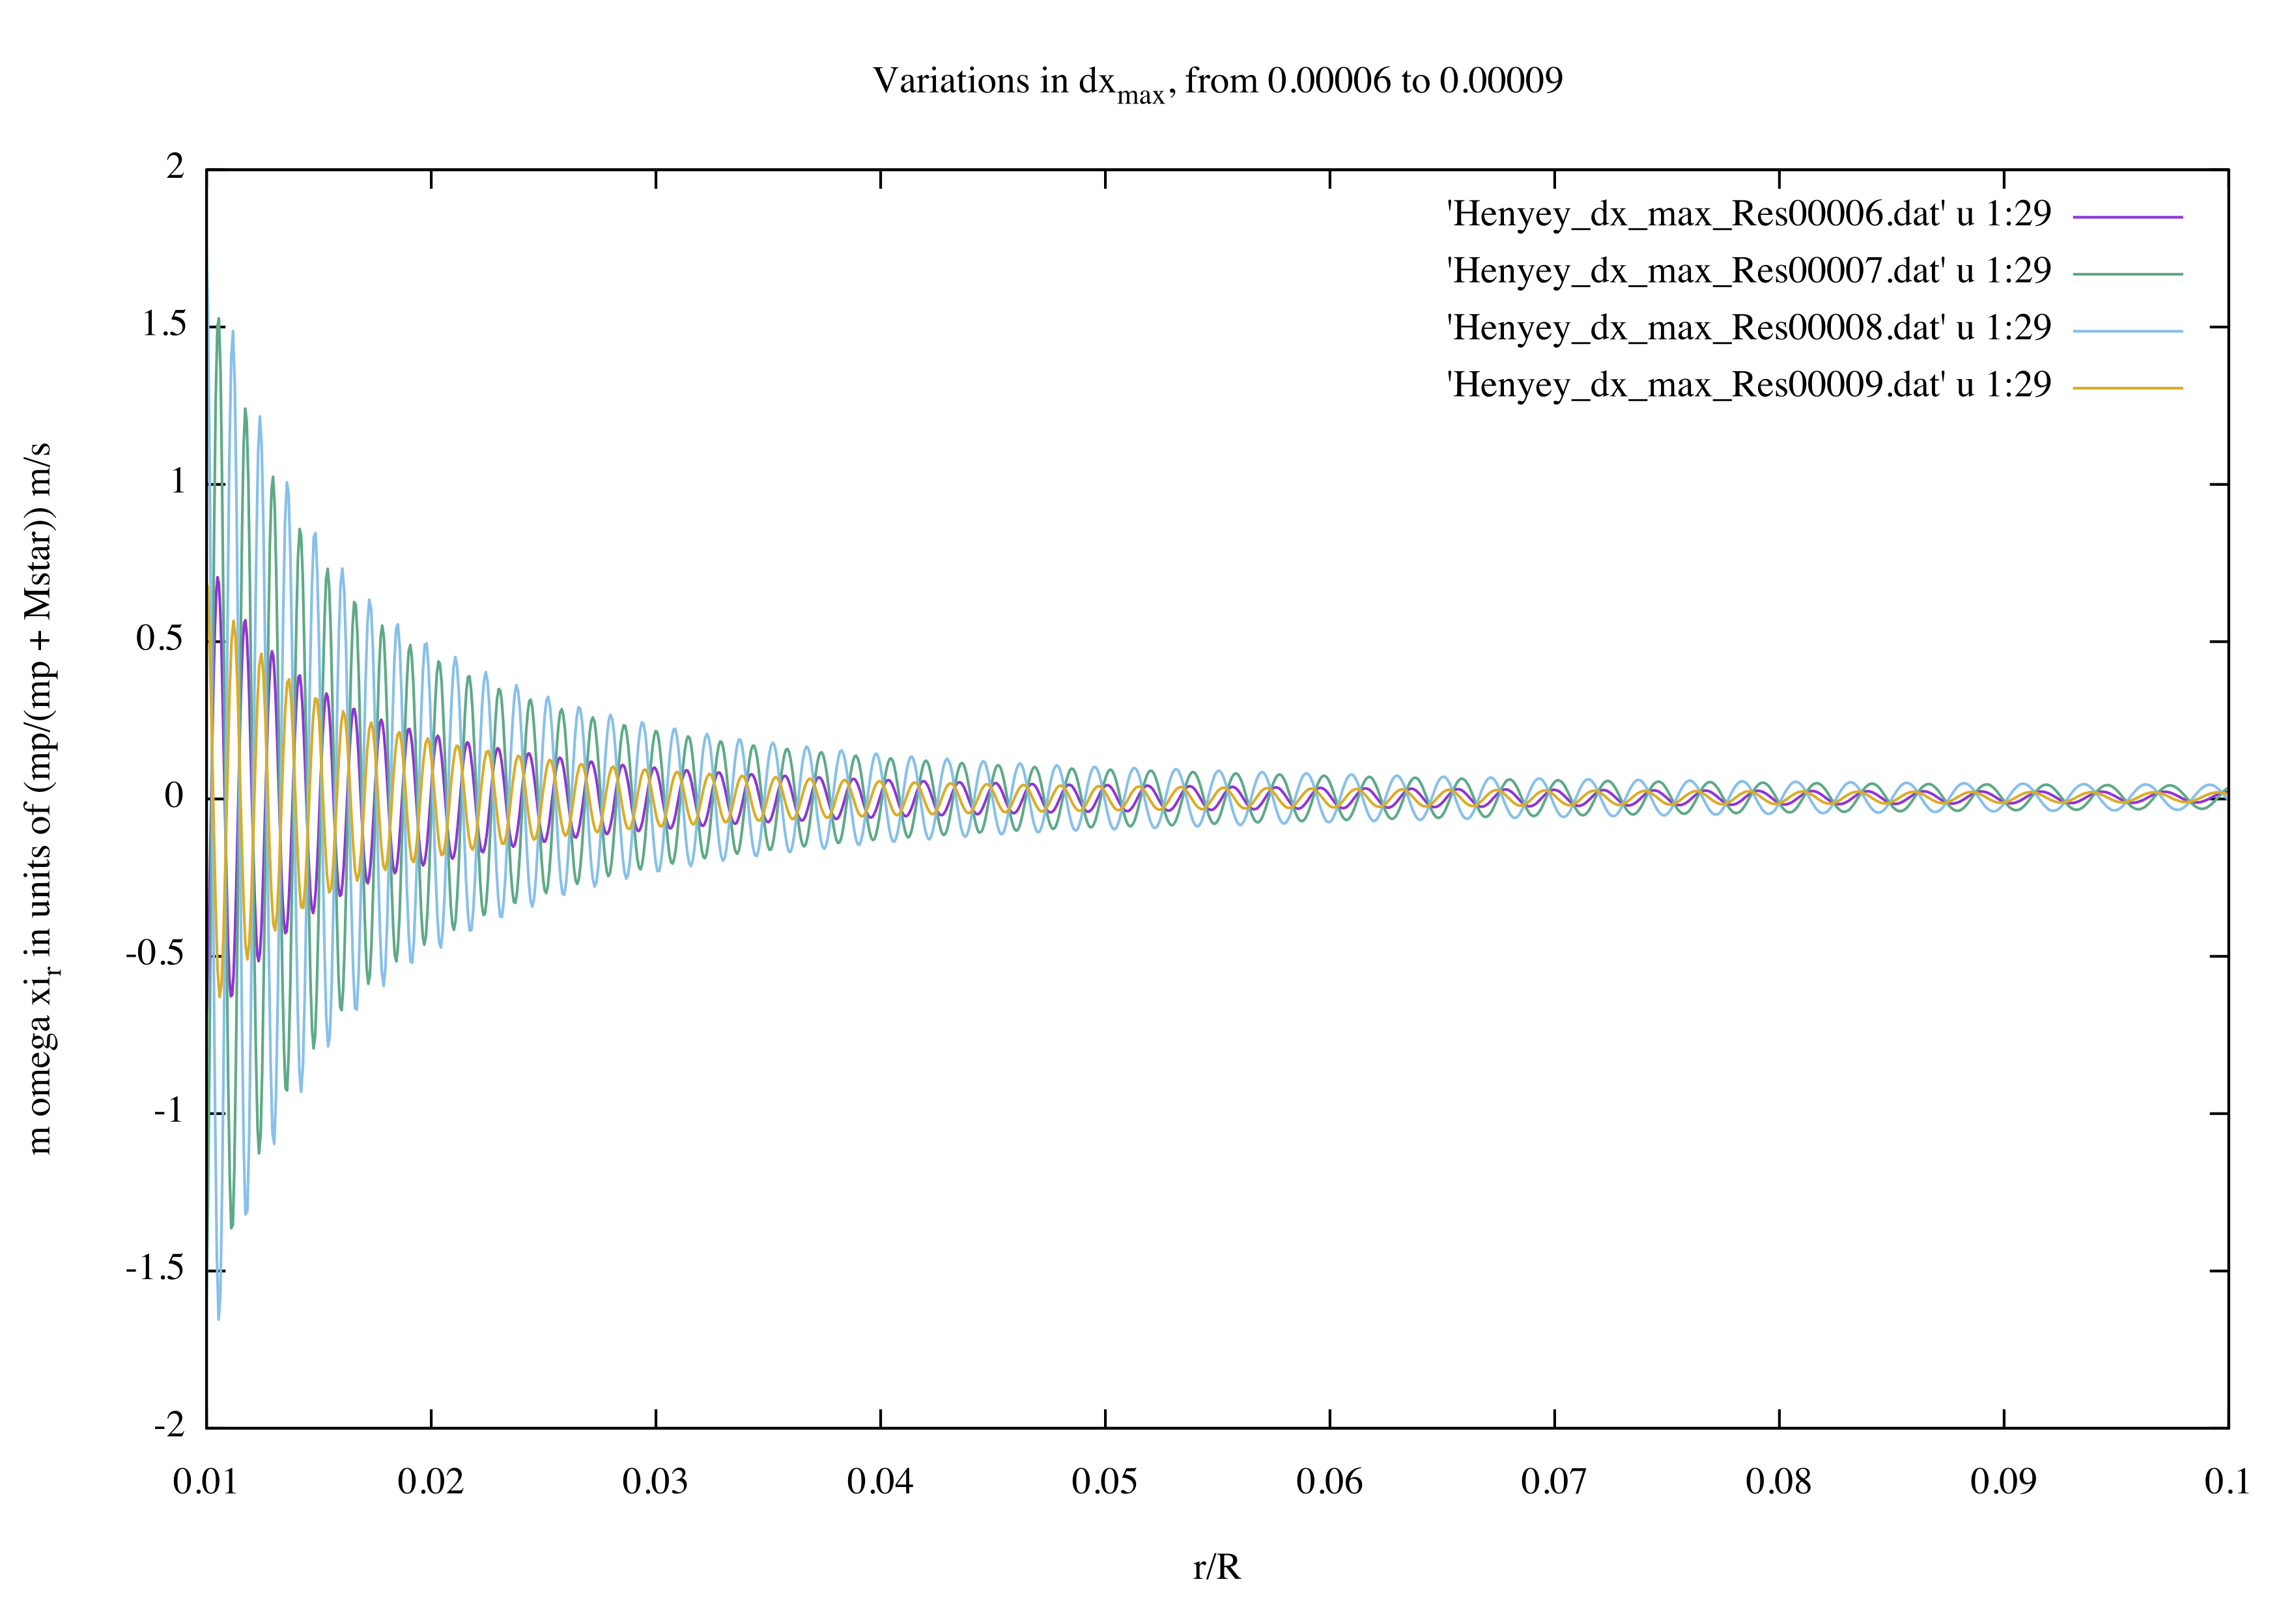
\includegraphics[width = \textwidth]{figures/xi_r_section2_Resvar.png}
\end{subfigure}

\begin{subfigure}{0.5\textwidth}
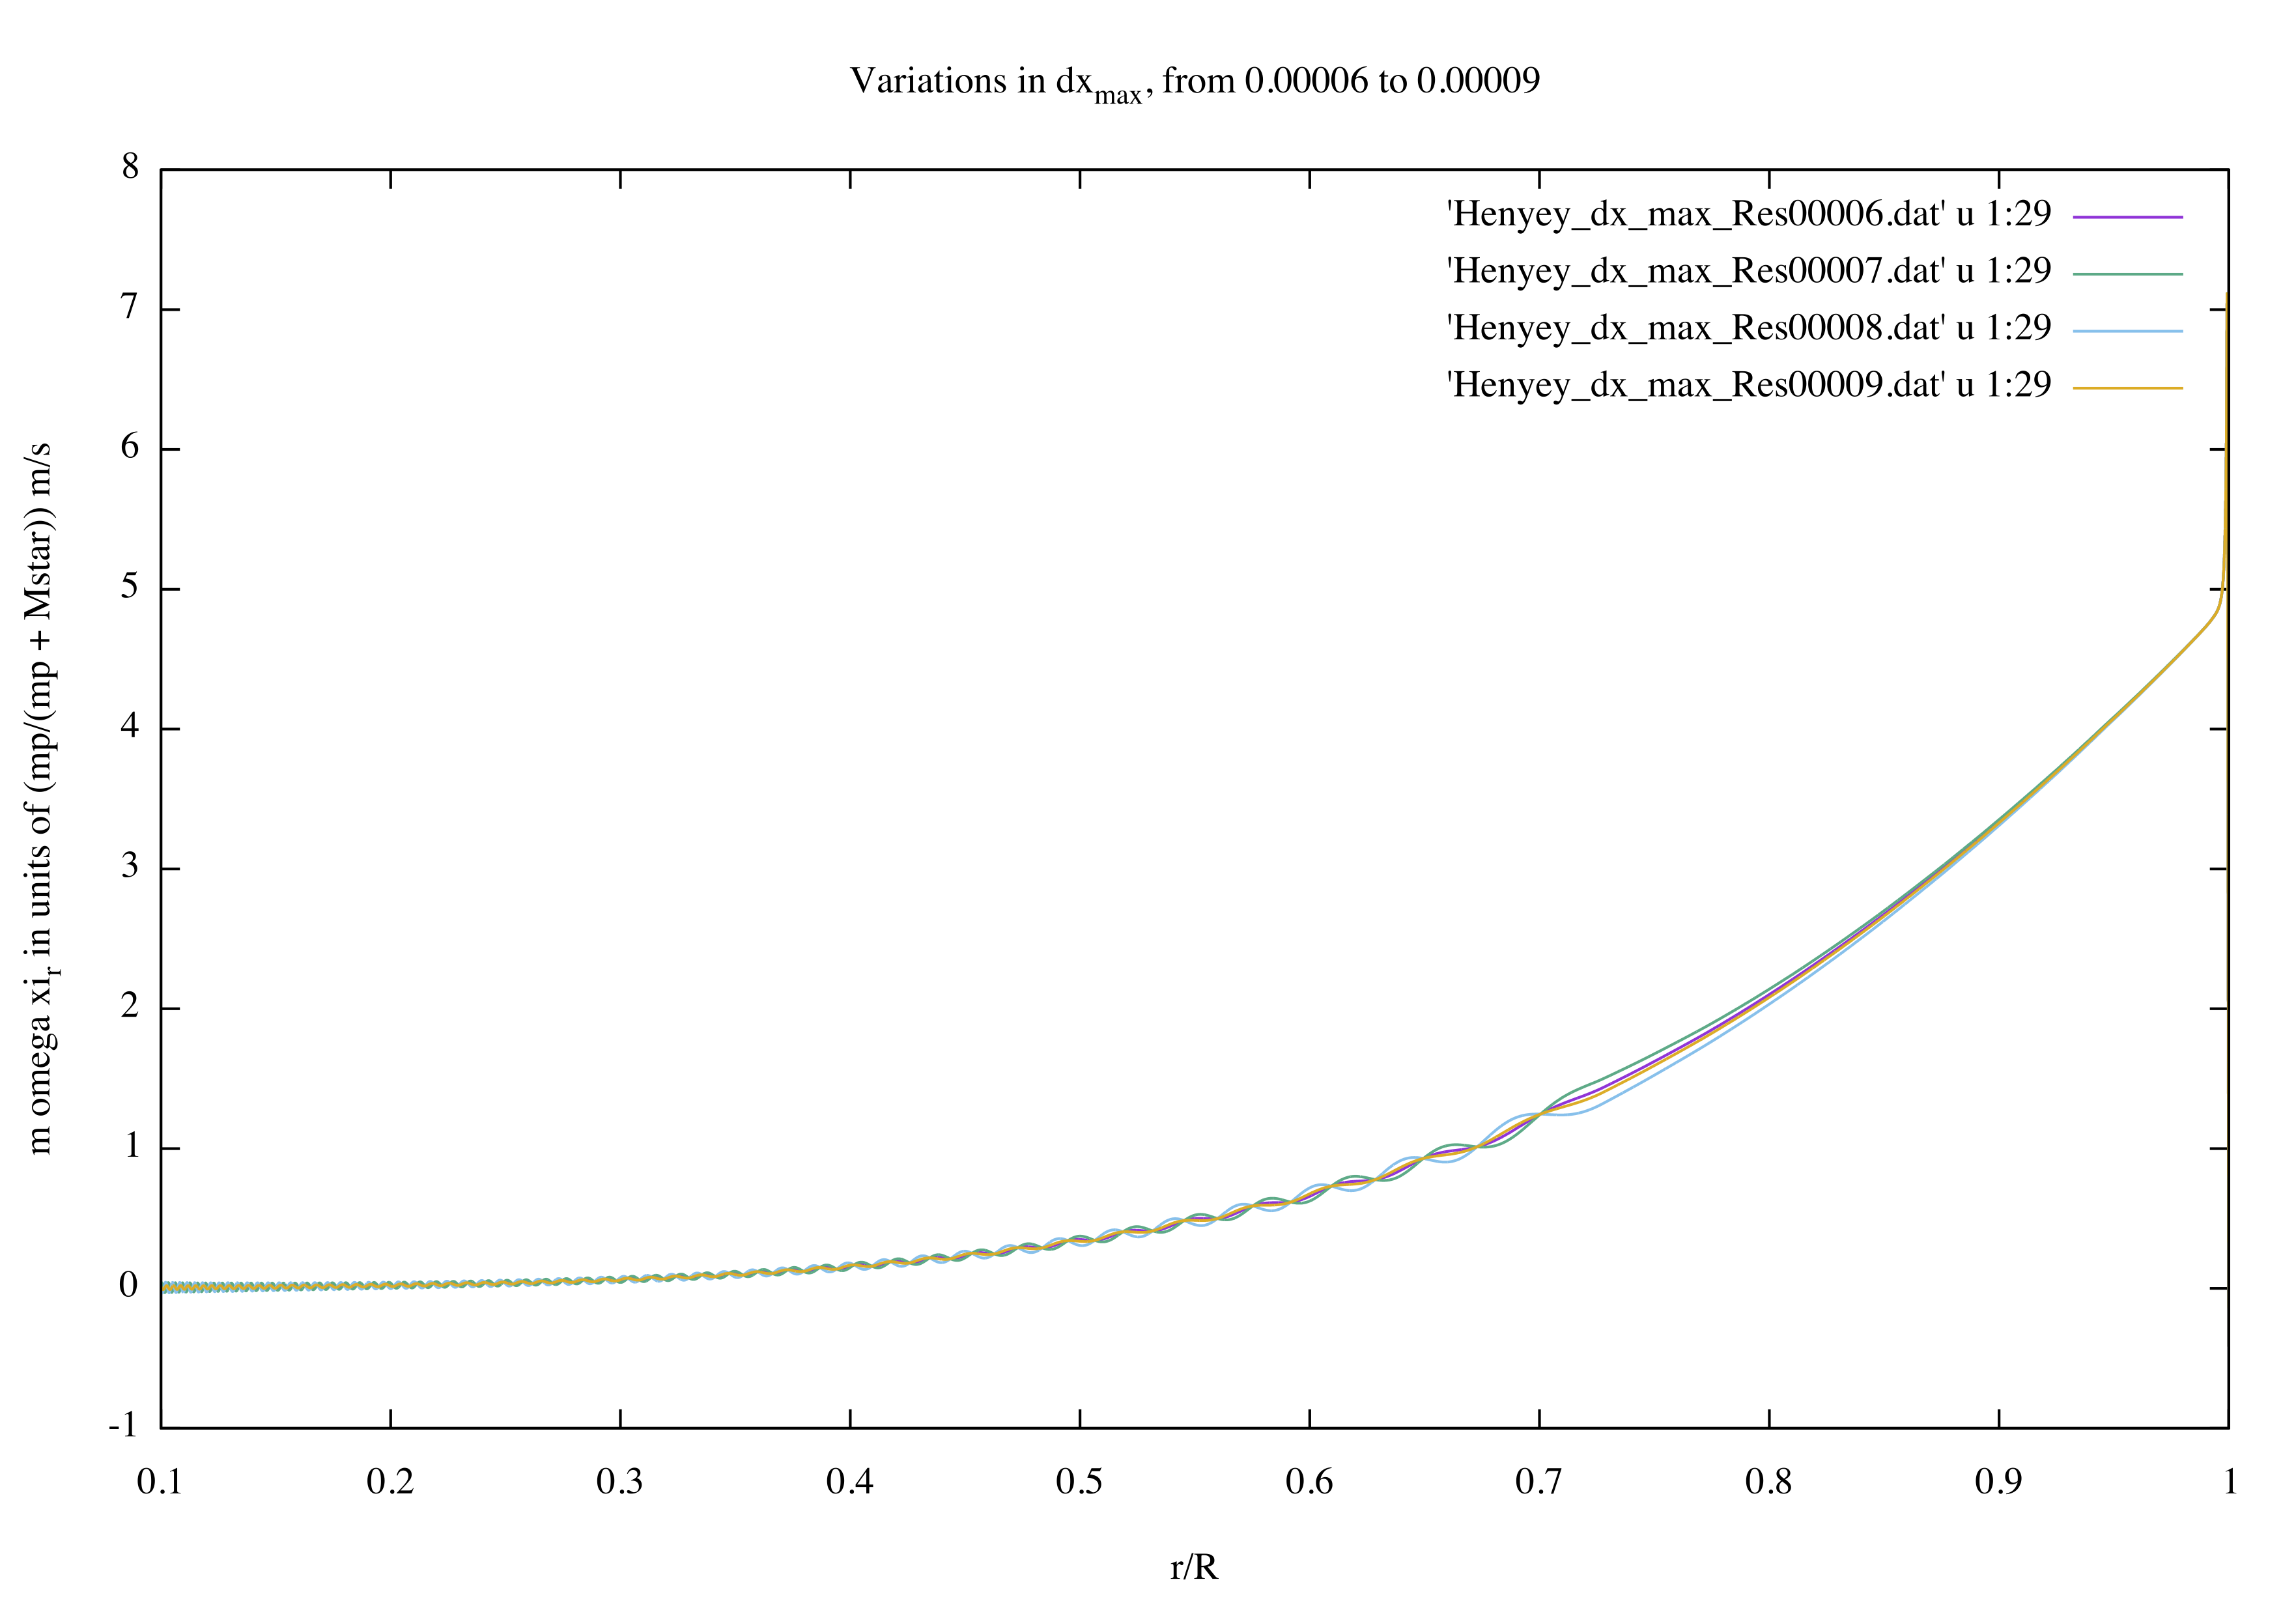
\includegraphics[width = \textwidth]{figures/xi_r_section3_Resvar.png}
\end{subfigure}
~
\begin{subfigure}{0.5\textwidth}
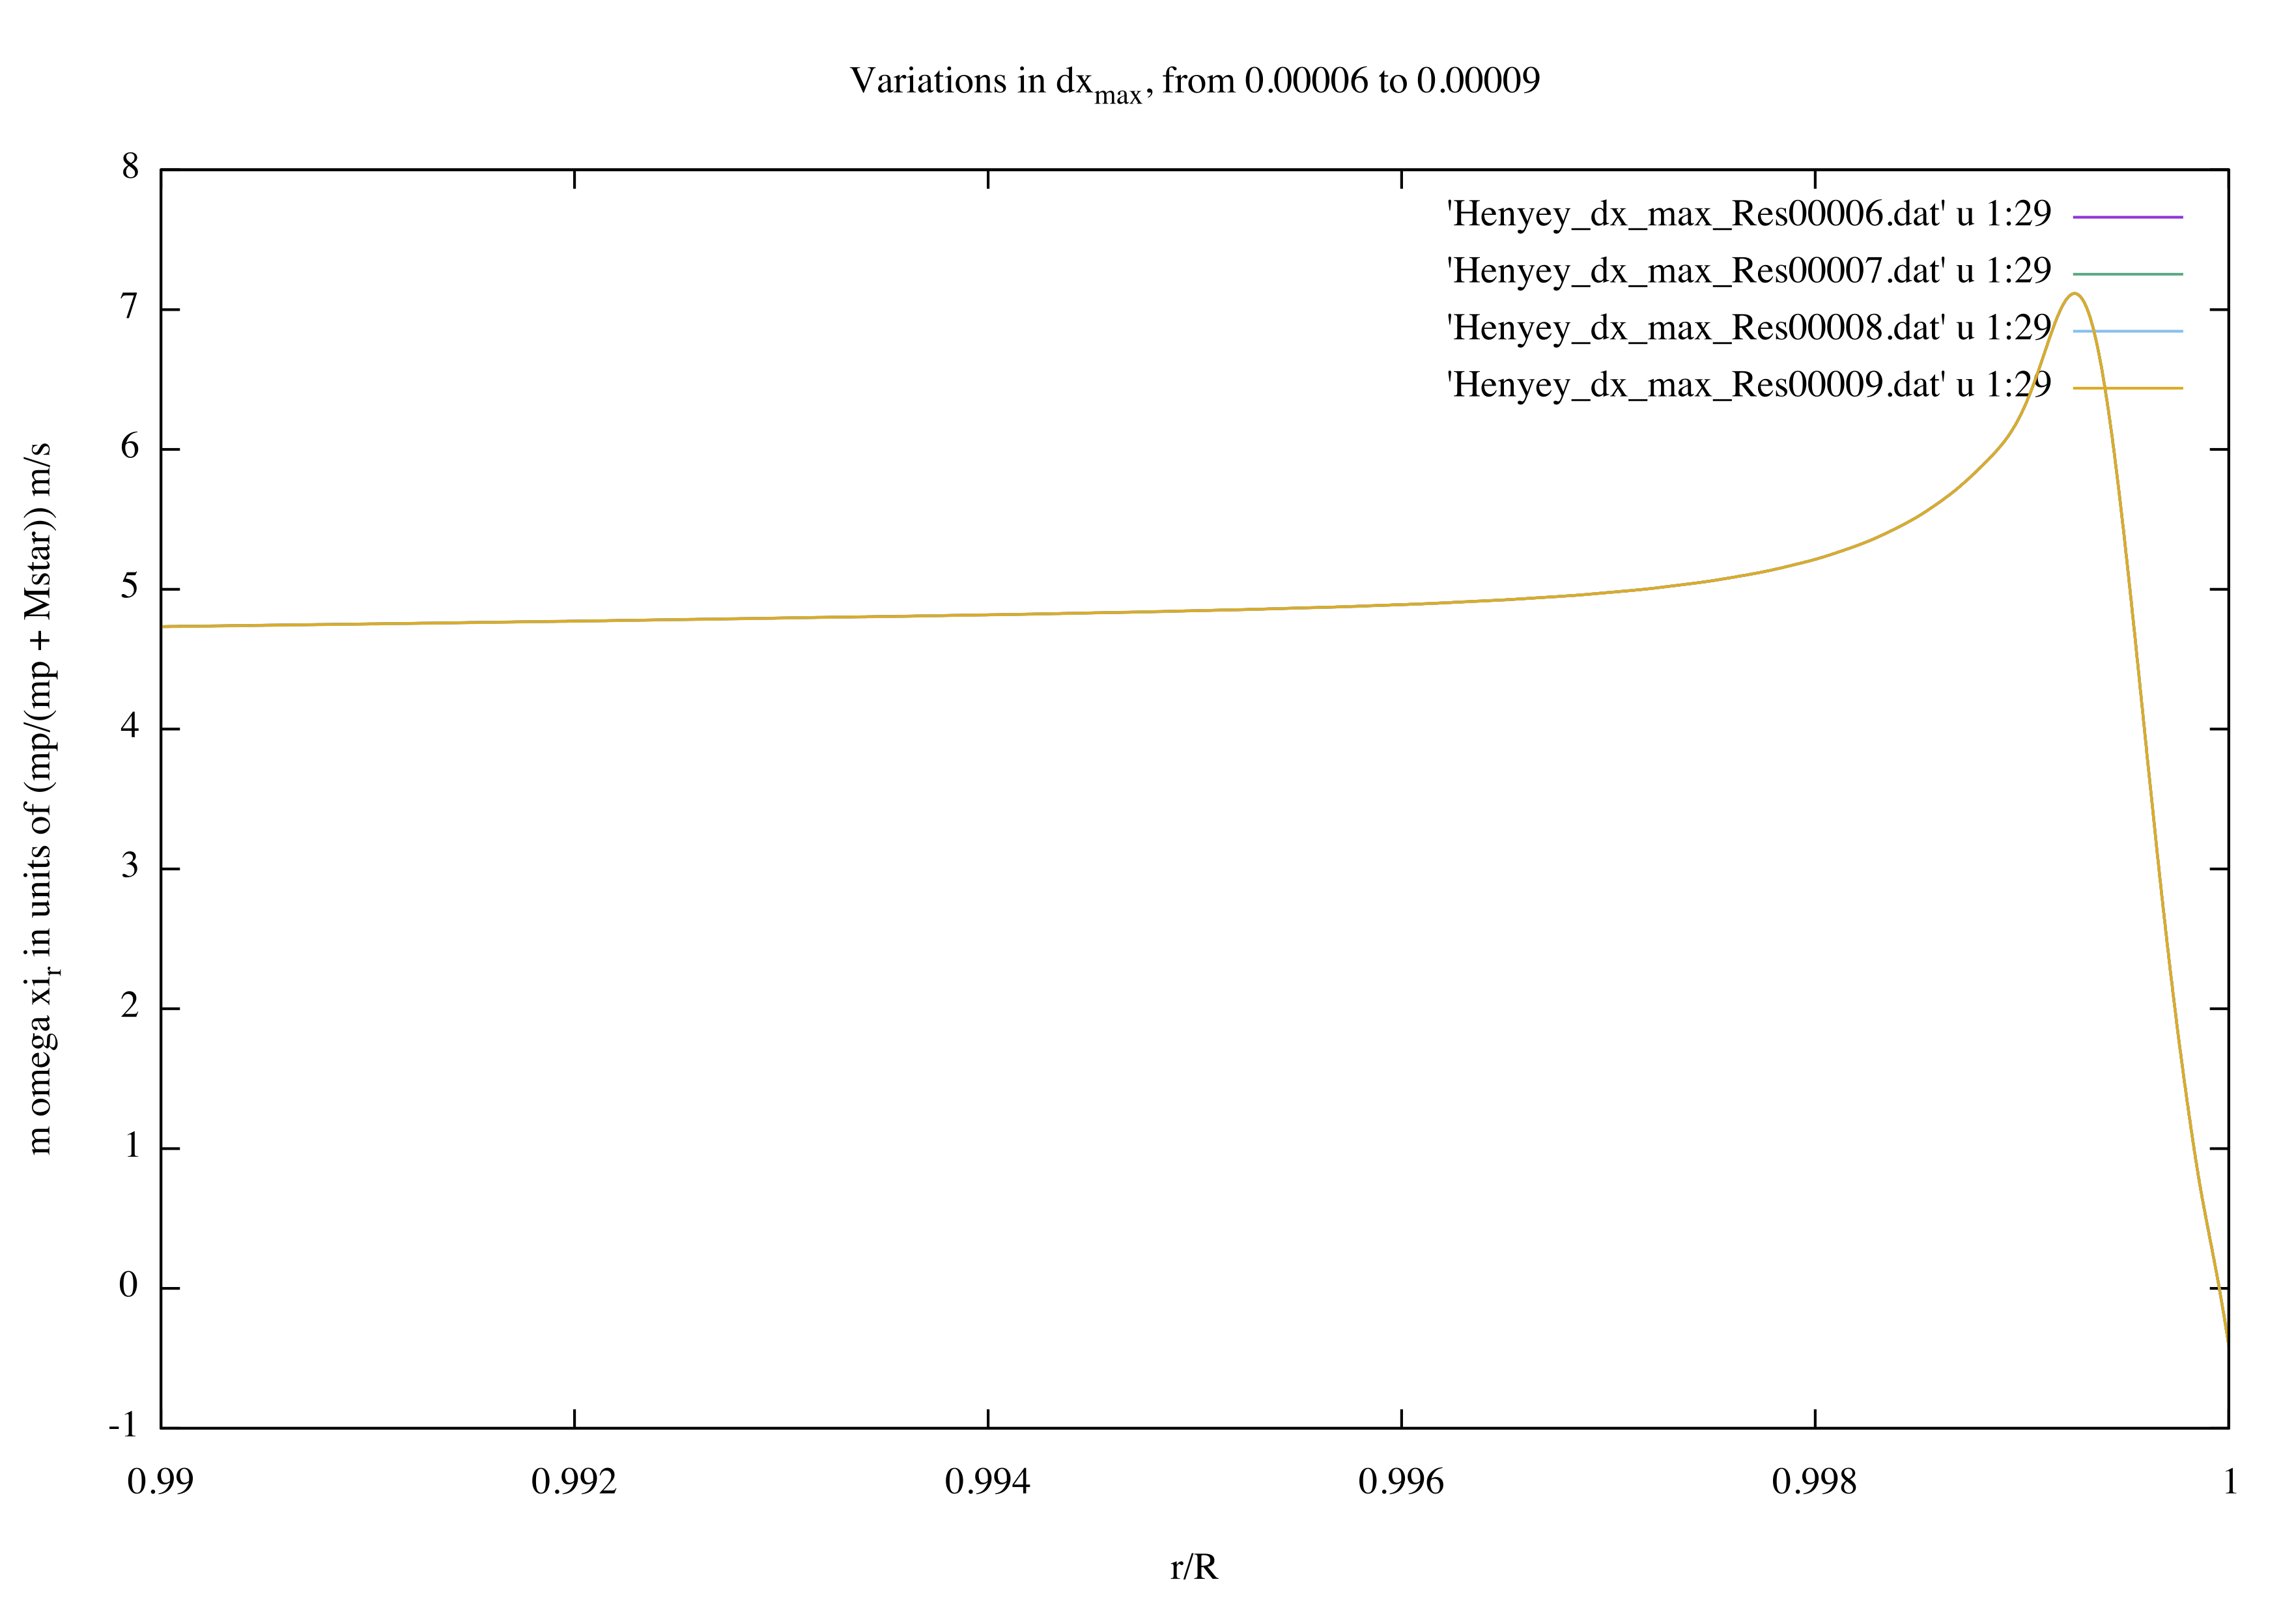
\includegraphics[width = \textwidth]{figures/xi_r_surface_Resvar.png}
\end{subfigure}

\caption{The full solution for the non-adiabatic case, showing the peak radial velocity (that is, $m \omega \xi_{r}$) in units of $\frac{m_{p}}{m_{p} + M_{*}}$ m s$^{-1}$, against the proportional radial distance from the centre.  In these figures the maximum cell size, and therefore the resolution limit of the grid, has been varied slightly, leading to a spread in the amplitudes of the oscillations.  The maximum cell size, as a proportion of the stellar radius, is plotted at $6 \times 10^{-5}$ (purple line), $7 \times 10^{-5}$ (green line), $8 \times 10^{-5}$ (blue line), and $9 \times 10^{-5}$ (orange line).}
\label{fig:Dvar}
\end{center}
\end{figure}




\section{Acknowledgements}  \label{Acknowledgements}

I would like to acknowledge MESA, \cite{Paxton2011}. http://mesa.sourceforge.net/index.html

This research has made use of the NASA Exoplanet Archive, which is operated by the California Institute of Technology, under contract with the National Aeronautics and Space Administration under the Exoplanet Exploration Program.





\bibliographystyle{plain}
\bibliography{library}









\newpage

\appendix

\section{Stellar Oscillation Equations} \label{ap:Osc}


\section{Detailed explanation of the general Henyey Method}   \label{ap:Henyey}




\end{document}  
